\documentclass[12pt]{article} 

\usepackage[right = 3.0cm, top = 3.5cm, bottom = 3.5cm, left = 3.0cm]{geometry}

\usepackage[english]{babel}
\usepackage[T1]{fontenc} % este y el de abajo son importantes para las tildes en acentuación

\usepackage{float} % for floating environments
\usepackage{stmaryrd, amsfonts, amssymb, amsmath, amsthm, mathrsfs, mathtools} % for mathematical symbols and equations, and other things
\usepackage{epsfig, graphicx, subfigure} % for inserting figures
\usepackage{caption, subcaption} % for adjusting captions of tables and figures
\usepackage{color} % for writing colored texts
\usepackage{setspace} % for adjusting line spacing
\usepackage{titlesec} % for theorem´s enumeration, etc.
% \usepackage{bbm} % for using \mathbbm{1}
\usepackage{url} % tú que crees
\usepackage{bbm} % para usar \mathbbm{1}
\usepackage{comment} % for comment text

\usepackage{makeidx} % no sé, no me acuerdo

% \usepackage{mdframed}
% % Define theorem environment inside a box
% % Define boxed theorem environment
% \newmdtheoremenv[
%   linecolor=black,
%   linewidth=0.5pt,
%   backgroundcolor=white,
%   innertopmargin=5pt,
%   innerbottommargin=7pt
% ]{theorem}{Theorem}[section]

% \newmdtheoremenv[
%   linecolor=black,
%   linewidth=0.5pt,
%   backgroundcolor=white,
%   innertopmargin=5pt,
%   innerbottommargin=7pt
% ]{proposition}{Proposition}[section]

% \newmdtheoremenv[
%   linecolor=black,
%   linewidth=0.5pt,
%   backgroundcolor=white,
%   innertopmargin=5pt,
%   innerbottommargin=7pt
% ]{lemma}{Lemma}[section]

% \newmdtheoremenv[
%   linecolor=black,
%   linewidth=0.5pt,
%   backgroundcolor=white,
%   innertopmargin=5pt,
%   innerbottommargin=7pt
% ]{conjecture}{Conjecture}[section]

% redefiniéndolos para que se enumeren según las secciones
\theoremstyle{plain} % in italic
\newtheorem{theorem}{Theorem}[section]
\newtheorem{lemma}[theorem]{Lemma}
\newtheorem{proposition}[theorem]{Proposition}
\newtheorem{conjecture}[theorem]{Conjecture}
\theoremstyle{definition} % normal
\newtheorem{definition}[theorem]{Definition}
\newtheorem{remark}[theorem]{Remark}

\def\<#1>{\mathinner{\langle#1\rangle}}

\usepackage{tikz}
\usetikzlibrary{graphs, graphs.standard, quotes, shapes.geometric}
\usepackage{ifthen}

\tikzset{costLine/.style={ultra thin, line width=0.5pt, color=blue}}

\newcommand{\costOne}{
    \begin{tikzpicture}[baseline, yshift=0.5ex]
        \draw[costLine] (0, 0) -- (1, 0);
    \end{tikzpicture}
}

\newcommand{\costZero}{
    \begin{tikzpicture}[baseline, yshift=0.5ex]
        \draw[dashed, costLine] (0, 0) -- (1, 0);
    \end{tikzpicture}
}
\definecolor{blue(pigment)}{rgb}{0.2, 0.2, 0.6}

\newcommand\norm[1]{\left\lVert#1\right\rVert}

% para el paseudocódigo
\usepackage{algorithm}
\usepackage{algorithmic}

% para que los hyperlinks no tengan color
\usepackage[colorlinks=false]{hyperref} % links

% for the E of the probability space, \mathcal{E}
% \usepackage{boondox-cal}

% redefining some math commands
\newcommand{\R}{\mathbb{R}}
\newcommand{\Z}{\mathbb{Z}}
\newcommand{\N}{\mathbb{N}}
\newcommand{\C}{\mathbb{C}}
\newcommand{\E}{\mathbb{E}}
\newcommand{\Pbb}{\mathbb{P}}
\newcommand{\F}{\mathscr{F}}
\newcommand{\Lip}{\text{Lip}}

% command for the projection of a vector 1 onto a vector 2
\DeclareMathOperator{\proj}{proj}
\newcommand{\vct}{\mathit}
\newcommand{\vectproj}[2][]{\proj_{\vct{#1}}[\vct{#2}]}

% for the fill square in the end of the proofs
\renewcommand{\qedsymbol}{\ensuremath{\blacksquare}}
\renewenvironment{proof}{{\bfseries Proof.}}{\qed}

\newenvironment{someideasfortheproof}{%
  {\bfseries Some ideas for the proof.}%
}{%
  \qed
}


% for the special arrows in the description of the examples
\makeatletter
\newcommand{\fixed@sra}{$\vrule height 2\fontdimen22\textfont2 width 0pt\shortrightarrow$}
\newcommand{\shortarrow}[1]{%
  \mathrel{\text{\rotatebox[origin=c]{\numexpr#1*45}{\fixed@sra}}}
}
\makeatother

% spacing between parragraphs and before its start
%\parindent = 0mm % no deja sangría
\setlength{\parindent}{1em} % deja sangría
\setlength{\parskip}{6pt} % Espacio entre párrafos


\title{\Large Percolation games: percolation structures in two non-oriented examples on $\Z^2$ and random transitions in oriented games}
\author{Melissa González García under the supervision of Bruno Ziliotto}
\date{}

% \newcommand\norm[1]{\left\lVert#1\right\rVert}

\begin{document}
	\maketitle
	\vspace{-1.5cm}
	\begin{center}
		Internship report, Research Master 2 MATH, Applied and Theoretical Mathematics\\
	 	Université Paris Dauphine PSL, CEREMADE, August 2024
 	\end{center}
 	

	\vspace{1.0cm}
	\begin{abstract}
		Percolation games are a class of zero-sum stochastic games in which a token moves across $\Z^d$ based on a transition function jointly controlled by both players, with random, spatially distributed payoffs. When the payoffs are i.i.d. in space and the game is oriented --meaning the token tends to move in a fixed direction regardless of the players' actions-- the value of the $n$-stage game has been shown to converge to a limit as $n$ tends to infinity. It remains unresolved whether this convergence occurs without the orientation assumption. This research explores this question by first analyzing two examples on $\Z^2$, whose limit values turn out to be directly related to percolation through specific lattice structures that provide strategic advantages to the players. We geometrically characterize these structures, analyze the critical probabilities of their occurrence, and explore their strategic implications. Computational simulations offer additional insights. Secondly, we extend the percolation games model by incorporating a stochastic process into the first component of the state transitions. This modification allows the token in an oriented game to return to previously visited states. For an i.i.d. and oriented game, if the stochastic process has a mean of zero, the resulting game preserves orientation in expectation. Moreover, if it also has bounded support, we prove that the game possesses a limit value, with its expected value converging at the same rate as that of the base game, thus extending the original result.
	\end{abstract}
	\thispagestyle{empty}

	\newpage
	\tableofcontents

	% sections
	\section{Introduction}
	In a \emph{zero-sum game}, two players choose their strategies simultaneously and receive opposite payoffs. The central solution concept in zero-sum games is the \emph{value}. Under standard assumptions, a minmax theorem \cite[Appendix A.5]{Sorin2002} guarantees the existence of the value and optimal strategies, which represent the outcome of the game played by rational players.

	\emph{Zero-sum stochastic games} generalize strategic-form games to dynamic situations and Markov Decision Processes (MDPs) to competitive scenarios. Introduced by Lloyd Shapley \cite{Shapley1953}, their seminal model involves two players who repeatedly play a zero-sum game that depends on a variable called \emph{state}. The state evolves stochastically from one stage to the next, based on the players' actions and the previous state. At each stage, players know the current state and each other's past actions. For a given initial distribution and $n \in \N$, the \textit{$n$-stage game} is defined, where player 1 aims to maximize the expected average payoff over $n$ stages, and player 2 aims to minimize it. The $n$-stage game has a value, denoted by $v_n$. A key question is the convergence of $v_n$ as $n$ tends to infinity, i.e., the study of the long-duration game (see, for example, \cite{LarakiSorin2015} for a comprehensive exposition). Bewley and Kohlberg \cite{BewleyKohlberg1976} proved the existence of the \emph{limit value} for zero-sum stochastic games with finite state spaces and action sets, which can be seen as an approximate payoff solution of the game as the number of stages tends to infinity. Following this seminal work, among the long stream of works studying this question, counterexamples for infinite state spaces and/or action sets have been identified (see, e.g., \cite{Vigeral2013, Ziliotto2016}).

	Recently, the \emph{Percolation Games} model \cite{GarnierZiliotto2022} was introduced as a new model of zero-sum stochastic games with an infinite state space. In a \textit{percolation game}, two players move a token along the edges of $\mathbb{Z}^d$, with the payoff function being random in space and known in advance by the players. For a given initial state $z \in \mathbb{Z}^d$, the $n$-stage game is defined as the game where the payoff is the (random) average payoff over $n$ stages. It has been proven that for i.i.d. and \textit{oriented} percolation games, $v_n$ converges almost surely to a limit value as the duration tends to infinity. Here, ``oriented'' refers to games where the object tends to move in a fixed direction regardless of players' actions, and ``i.i.d.'' indicates that the payoff function is independent and identically distributed in space. As previously noted, studying the existence of the limit value is particularly challenging in stochastic games with infinite state spaces. Thus, the interest in this model, which despite having an infinite state space has a lot of structure.

	This model also connects with classic percolation problems, such as first passage and last passage percolation. Essentially, studying the average minimal or maximal cost to traverse a distance $n$ can be reformulated as a one-player game. This model goes one step further by adding another player. Additionally, it provides a discrete-time stochastic game framework \cite[Section 4]{GarnierZiliotto2022} suitable for studying the \textit{non-convex stochastic homogenization} of Hamilton-Jacobi equations \cite{LionsPapanicolaouVaradhan1987}. Very briefly, there is an analogy between the existence of a limit value in percolation games and the existence of an asymptotic value in continuous-time games where the environment evolves according to a differential system controlled jointly by the players, known as \textit{differential games}, which value functions are solutions to Hamilton-Jacobi equations. This connection has been explored in \cite{Ziliotto2016, FeldmanFermanianZiliotto2021}, whose authors provide examples of non-convex Hamilton-Jacobi equations that do not homogenize in a stationary ergodic environment, inspired by stochastic games with state space $\mathbb{Z}^2$ that lack a limit value.

	A natural and still open question for percolation games is whether the limit value exists without the orientation assumption. In the i.i.d. setting, the existence of the limit value is not guaranteed without this assumption, and even when it does exist, it may be random and dependent on the initial state. Studying this question presents a significant challenge, as the value can strongly depend on local properties of the environment in the absence of orientation. During this research internship, our goal was to delve a little deeper into this question by examining specific non-oriented games.
	
	First, we studied two examples in which players move a token along the vertices of the square lattice $\Z^2$, incurring the cost associated with each edge traversed, with edge costs being i.i.d. Bernoulli random variables. The main difference between them is that in the first game, the token moves only once at each stage as a result of the combined actions of both players, while in the second game, the token moves twice --once for each player's action. 
	% The first game is non-symmetric, while the second game is symmetric. 
	This part of the study is motivated by a research conducted by Ziliotto \cite{Ziliotto2023}, who, together with Avelio Sepúlveda, has worked on characterizing the critical probability of oriented bond percolation through the limit value of the first game. They proved that for this game, the limit value is independent of the initial state and deterministic, further establishing that it is 1 if and only if the Bernoulli parameter exceeds the critical probability threshold for oriented bond percolation. This motivated us to explore the conditions under which the limit value might be 0 and to investigate the second game, seeking to uncover potential connections with percolation theory.

	In analyzing these games, we focused on percolation through specific lattice structures that confer strategic advantages to the players. These structures, along with their associated critical probabilities, are crucial for devising optimal gameplay strategies. For the first game, we provided a geometric characterization of the advantageous structure for player 1, corresponding to a value of zero (since player 1 aims to minimize), and demonstrated the non-triviality of its critical probability. For the second game, we employed a similar approach and attempt to prove that its limit value is also independent of the initial state and deterministic. Additionally, we established a geometric characterization of the advantageous structures for each player and showed that their critical probabilities are non-trivial. We formulated several conjectures that, while strongly believed to be true, we were unable to prove conclusively. To test these conjectures and gain further insights, we conducted computational simulations for both games. This approach was particularly valuable for the second game, where simulations significantly enhanced our understanding. In this game, the distribution of 0s and 1s across the structures emerged as a significant factor.

	In the second part of our work, we extended the original i.i.d. and oriented percolation games by introducing a stochastic process into the first component of the game's state transitions. This modification allows the token to return to previously visited states while remaining oriented in expectation, provided the stochastic process has a mean of zero. We then analyzed the value of this new game and proved that if the stochastic process also has bounded support, the resulting game possesses a limit value and that its expected value has a rate of convergence which, up to a constant factor, is equal to that of the original percolation game.

	In the following section, we provide a formal description of the Percolation Games model and summarize all relevant aspects and known results. In Section 3, we present the two examples and the theoretical analysis conducted, followed by a description of the computational methods used and a discussion of the results obtained. In Section 4, we introduce the generalized model mentioned above and prove our main result. Finally, in Section 5 we conclude and give our perspectives for future work.


	\subsubsection*{Notations} The set of nonnegative integers is denoted by $\N$, and by $\N_+ := \N \setminus \{0\}$. The set of real numbers is denoted by $\R$ and by $\bar{\R} := \R \cup \{+\infty, -\infty\}$.

	The set of integers is denoted by $\Z$ and by $\Z^d := \{(x_1, x_2, \ldots, x_d) : x_i \in \Z, \text{for } i =  1, 2, \ldots, d\}$. We turn $\Z^d$ into a graph by adding an (undirected) edge between every pair of vectors $x$ and $y$ such that $|x - y| = 1$. The resulting set of edges is denoted by $\E^d$. In this context, we refer to the vectors in $\Z^d$ as vertices. The origin of this graph is the vertex $0 = (0, 0, \ldots, 0)$. 

	The square lattice rotated $45^\circ$ is denoted by $\Z^2_{r}$, and its edge set by $\E_r^2$.

	For $x, y \in \Z^d$, we write $x \leq y$ if $x_i \leq y_i$ for $1 \leq i \leq d$, and we let $\vec{\mathbb{L}}^d = (\Z^d, \vec{\mathbb{E}}^d)$ denote the directed graph obtained by assigning an arrow from $x$ to $y$ whenever $\{x, y\} \in \E^d$ and $x \leq y$.

	For $a, b \in \Z$, we denote $[a..b] := \{i \in \Z : a \leq i \leq b\}$, and for $n \in \N_+$, $[n] := [1..n]$.

	For a vector $\mathbf{v} = (v_1, v_2, \ldots, v_d) \in \R^d$, its $k$-th component is denoted as $[\mathbf{v}]_k := v_k$, and $\|\mathbf{v}\|$ represents its Euclidean norm.

	% For vectors $\mathbf{a}$ and $\mathbf{b}$ in $\R^d$, the vector projection of $\mathbf{a}$ onto  $\mathbf{b}$ is denoted as $\vectproj[\mathbf{b}]{\mathbf{a}}$.

	Let $f, g$ be real functions. If $f(x)$ is big-O of $g(x)$ as $x$ tends to $\infty$, we write $f(x) = O(g(x))$.

	Given a graph $G =(V, E)$, a \emph{percolation configuration} $\omega = (\omega_e \colon e \in E)$ is an element of $\{0, 1\}^E$. If $\omega_e = 1$, the edge $e$ is said to be \emph{open}; otherwise, $e$ is said to be \emph{closed}. A \emph{percolation model} is defined by a distribution on percolation configurations on $G$. 

	The simplest example of a percolation model is \emph{Bernoulli percolation} (also known as bond percolation), in which each edge is open with probability $p$ and closed with probability $1-p$, independently of the states of other edges. Another model is \emph{site percolation} in which the sites (or vertices) of the lattice are open or not, with probability $p$ and $1 - p$, respectively.

	We will consider Bernoulli percolation on the lattice $\Z^d$, $\Z_r^d$ and $\vec{\mathbb{L}}^d$, the latter of which is known as \emph{oriented bond percolation}. For each graph, with it corresponding configuration space $\{0, 1\}^E$, we associate the $\sigma$-algebra $\F$ generated by events depending on finitely many edges. For $0 \leq p \leq 1$, we let $\Pbb_p$ denote the corresponding product measure on $(\{0, 1\}^E, \F)$ with density $p$. 	
	\section{Percolation Games}
	The Percolation Games model was introduced by Garnier and Ziliotto in \cite{GarnierZiliotto2022}. In their paper, they define i.i.d. and oriented percolation games, and for them show that as $n$ tends to infinity, the sequence of values of the $n$-stage game converges almost surely to a constant, and determine the rate of convergence of it expected value. They also prove that the assumption of i.i.d. is necessary for this result.

	The primary reference for this game model is their article, upon which we rely for writing this section. First, we describe the model and provide a brief overview of related models. Second, we present the main results regarding the existence of the limit value, as stated in their article.

	\subsection{Model}
	A percolation game is a zero-sum stochastic game with state space $\Z^d$, for $d \geq 1$ and is described by a tuple $\Gamma = (I, J, \mathcal{E}, g, q)$, where 
	\begin{itemize}
		\item[-] $I$ and $J$ are finite sets representing respectively player 1’s and player 2’s action sets.
		\item[-] $\mathcal{E} = (\Omega, \F, \Pbb)$ is a probability space equipped with a collection of measurable transformations $\{\tau_z\}_{z \in \mathbb{Z}^d}$ that map $\Omega$ to itself, which are measure-preserving and form a group under composition, i.e.
		\[
			\Pbb(\tau_z(F)) = \Pbb(F) \; \text{ and } \; \tau_{z+z'} = \tau_z \circ \tau_{z'}, \text{ for all } z, z' \in \Z^d \text{ and } F \in \F.
		\]
		Moreover, the transformations ${\tau_z}$ are assumed to be ergodic: any event $F \in \F$ that is invariant (i.e., $\tau_z(F) = F$ for all $z \in \mathbb{Z}^d$) must have probability 0 or 1. 

		\item[-] $g := \{\omega \mapsto g_{\omega}(z,i,j)\}, (z,i,j) \in \Z^d \times I \times J$ is a collection of real-valued random variables defined on $\Omega$, uniformly bounded and stationary, i.e. 
		\[
			g_{\tau_z(\omega)}(z', i, j) = g_{\omega}(z + z', i, j), \text{ for all } (z, z', i, j).
		\]
		\item[-] $q \colon I \times J \to \Z^d$ is a function that determines the transition between states. It is referred to as the transition function of the game.
	\end{itemize}

	The transformations $\tau_z$ are just translations of the lattice by $z \in \Z^d$.
	
	Given some initial state $z \in \Z^d$ and $\omega \in \Omega$, the game proceeds as follows:
	\begin{itemize}
		\item[--] Players are informed of $\omega$.
		\item[--] At every stage $m \in \N_+$, both players are informed of the current state $z_{m}$. Player 1 chooses an action $i_m$ and then, knowing player 1's action, player 2 chooses an action $j_m$. The payoff at stage $m$ is $g_m^{\omega} := g_{\omega}(z_{m}, i_m, j_m)$, which represent the payoff of player 1, with player 2 receiving the opposite payoff. The new state $z_{m + 1}$ is then chosen according to $q(i_m, j_m)$ by  
		\[
			z_{m+1} := z_m + q(i_m, j_m).
		\]
		Then, the triplet $(i_m, j_m, z_{m+1})$ is publicly announced to the players.
	\end{itemize}

	\begin{remark}
		We could define $g$ as $\{\omega \mapsto (g_{\omega}(z,i,j))_{(i, j) \in I \times J}\}_{z \in \Z^d}$: for each $z$, there is a vector of random variables indexed by $(i, j)$. However, this definition imposes some structure on the original one. Indeed, it can be viewed as a particular case of the other, where the collection of random variables is organized in a specific manner. This definition might be useful when the cost on the edges is deterministic or when, for example, the payoffs are associated with the vertices rather than the edges.
	\end{remark}

	At every stage $m \in \N_+$, the information available to player 1 before playing is a vector of the form $(z, i_1, j_1, \ldots, z_{m-1}, i_{m-1}, j_{m-1}, z_m)$, and this is referred to as the history up to stage $m$. A strategy for player 1 is a sequence of mappings $\sigma = (\sigma_m)_{m\geq 1}$, such that $\sigma_m(h_{m}) \in I$ for every possible history $h_{m} \in (\Z^{d}\times I \times J)^{m-1} \times \Z^d$. Similarly, a strategy for player 2 is a sequence of mappings $\tau = (\tau_m)_{m \geq 1}$, where $\tau_m(h_m, i_m) \in J$ for all $(h_m, i_m) \in (\Z^{d}\times I \times J)^{m-1} \times \Z^d \times I$. The interpretation is that, given the history $h_m$, the strategy $\sigma_m$ tells player 1 to play $i_m$. Knowing $h_m$ and $i_m$, the strategy $\tau_m$ then tells player 2 to play $j_m$.

	\begin{remark}
		This is primarily a point of clarification. Once $\omega$ is fixed, which can be interpreted as nature having randomly selected one of the games according to $\Pbb$, the two players observe the entire realization of the game before play begins. From this point onward, there is no further randomness in the game: the players see the realization and can adjust their strategies accordingly.
	\end{remark}

	The set of strategies for player 1 and 2 are denoted by $\Sigma$ and $T$, respectively. Given an  initial state $z_1 \in \Z^d$ and a pair of strategies $(\sigma, \tau)$, they induce a play, which is a sequence $(z_m, i_m, j_m)_{m\geq1}$.

	The $n$-stage game, denoted by $\Gamma_n^{\omega}(z)$, is the zero-sum game with strategy sets $\Sigma$ and $T$, and payoff function $\gamma_n^{\omega} \colon \Z^d \times \Sigma \times T \to \R$ defined by
	\[
		\gamma_n^{\omega}(z, \sigma, \tau) := \frac{1}{n}\sum_{m=1}^ng_m^{\omega}.
	\]
	The value of $\Gamma_n^{\omega}(z)$ exists (by Theorem I.2.4 in \cite{Mertens2015}; see, for example, Chapter IV of the same book) and is the real number $v_n^{\omega}(z)$ such that
	\[
		v_n^{\omega}(z) := \max_{\sigma \in \Sigma}\min_{\tau \in T} \gamma_n^{\omega}(z, \sigma, \tau) = \min_{\tau \in T}\max_{\sigma \in \Sigma} \gamma_n^{\omega}(z, \sigma, \tau).
	\]

	In the sequel, $v_n(z) \colon \mathcal{E} \to \R$ denote the random variable $\omega \mapsto v_n^{\omega}(z)$, where $\R$ is equipped with the Borel $\sigma$-algebra.
	
	Percolation games can be situated within the framework of random games, where the payoffs or structure are determined by a probability distribution rather than being fixed or deterministic. Generally speaking, such models consider a specific space of games (e.g., in normal-form, extensive-form, or repeated games), a natural probability measure over this space, and study the properties of games randomly selected according to this measure (see, e.g., Amiet et al. \cite{Amiet2021} and Flesch et al. \cite{Flesch2023} for recent results).

	A percolation game is, in fact, a random turn-based stochastic game: initially, $\omega$ is drawn from $\Pbb$, and then players play a turn-based stochastic game determined by $\omega$, where ``turn-based'' means that players take turns selecting their actions.

	\begin{remark}
		In the seminal model of stochastic games introduced by Shapley \cite{Shapley1953}, players simultaneously choose their actions. Turn-based stochastic games can be viewed as a particular case of (simultaneous) stochastic games. This can be achieved by introducing ``dummy'' actions (e.g., ``wait'' or ``pass'') for each player, defining their strategies such that they alternate between the dummy actions and the original action sets, and redefining the transition and payoff functions to operate every two stages.
	\end{remark}

	Recently, Holroyd et al. \cite{Holroyd18} and Bashin et al. \cite{Bashin23} studied a class of games on the square lattice $\mathbb{Z}^2$, also referred to as percolation games by their authors. In their percolation games, two opposing players take turns moving a token along the vertices of $\mathbb{Z}^2$ based on some allowed moves, typically a finite subset of directed edges. Each vertex  is randomly and independently assigned one of three states: trap, target, or open, with probabilities $p$, $q$, and $1-p-q$, respectively. A player who moves the token to a trap loses the game immediately, while moving the token to a target results in an immediate win. The authors are interested in the probability of a draw (i.e. neither player can force a win) for fixed $p$ and $q$. There are several contrasts between these two notions of percolation games. For instance, the methods for aggregating the payoff differ, resulting in distinct payoff functions. Additionally, in the stage games presented in \cite{Bashin23}, exactly one player makes a move in each round, whereas in \cite{GarnierZiliotto2022}, each round consists of a move by player 1 followed immediately by a move by player 2. Furthermore, the problems they address differ: the former focuses on the probability of a draw, while the latter is concerned with the limit value of the game.

	Percolation games have also been defined in environments other than $\Z^d$. For instance, very recently, in \cite{Attia2024} were introduced a type of percolation game called \emph{directed games}, where the state space is an acyclic directed graph over $\Z^d$. 

	% The paper provides a formal game-theoretic formulation of the problem and suggest how the payoff function of the corresponding $n$-stage zero-sum game could be defined, facilitating the discussion on the connection with the model of this section. In terms of payoff, this game can be analyze as: if a player moves a token into a target (respectively, a trap), she receives a payoff of +1 (respectively, –1), and if no traps or targets are ever visited, both players receive payoff 0. 

	\subsection{Known results}
	Before stating the main results of Garnier and Ziliotto, we need to introduce two key definitions for percolation games.

	\begin{definition}
		A percolation game $\Gamma = (I, J, \mathcal{E}, g, q)$ is oriented if there exists $u \in \Z^d$ such that, for all $(i, j) \in I \times J$, $q(i, j) \cdot u > 0$.
	\end{definition}

	An oriented game can be intuitively described as a type of game where, regardless of the players' actions, the coordinates of the state with respect to $u$ always increase. The rate of this increase may vary depending on the players' actions.

	\begin{definition}
		A percolation game $\Gamma = (I, J, \mathcal{E}, g, q)$ is i.i.d. if the random variables $\{\omega \mapsto g_{\omega}(z, i, j)\}_{(z, i, j) \in \Z^d \times I \times J}$ are i.i.d.
	\end{definition}
	
	%Note that when the game is i.i.d., it satisfies the assumed properties of stationarity and ergodicity outlined in the model.
 	
 	Next, we present their main result, establishing the existence of a limit value for percolation games that are i.i.d. and oriented.

	\begin{theorem}\label{theorem_iid_and_oriented_percolation_games}
		For a percolation game that is i.i.d. and oriented, and all $z \in \Z^d$, $v_n(z)$ converges $\Pbb$-almost surely to a constant $v_{\infty} \in \R$ as $n \to \infty$. Moreover, there exist real constants $A, B > 0$ such that for all $n \geq 1$, $z \in \Z^d$ and $\lambda \geq 0$,
		\[
			\Pbb\left(|v_n(z) - v_{\infty}| \geq \lambda + A\ln(n + 1)^{1/2}n^{-1/2} \right) \leq \exp(-B\lambda^2n)
		\]
		In particular, 
		\[
			|v_{\infty} - \E(v_n)| \leq A\ln(n + 1)^{1/2}n^{-1/2},
		\]
		which indicates that $\E(v_n)$ converges to $v_{\infty}$ at a rate of $O(ln(n)^{1/2}n^{-1/2})$.
	\end{theorem}

	The proof of this theorem can be found in the referenced article. It will be further clarified in the penultimate section, where we prove the same result for a slightly more general class of percolation games, using the same ideas to those employed in the proof of this theorem.

	% First, it is demonstrated that $v_n(z)$ concentrates around its expectation $\E(v_n)$. This step includes defining the orthogonal hyperplane to the direction vector $u$, considering their translations, and an auxiliary game with a payoff of 0 on these hyperplanes. A crucial inequality arises when counting the number of times these hyperplanes are crossed during the game. Then, a martingale structure with bounded differences is established,  allowing the application of Azuma's concentration inequality. Next, it is shown that $\E(v_n)$ converges to $v$. This involves working with inequalities, playing the game in blocks, and studying the subadditivity of $(n\E(v_n))_{n\geq 1}$. The convergence rate is derived through induction, starting from the the result obtained from playing in blocks. Finally, using the previously established results, it is proven that $v_n$ concentrates around $v_{\infty}$ as $n$ tends to infinity.

	\begin{remark} 
		As a by-product of the proof of the existence of $v_{\infty}$, it follows that $v_{\infty}$ is deterministic and independent of the initial state. This means that the outcome of the $n$-stage game converges to a deterministic result that is inherent to the dynamics of the game, rather than being influenced by the starting state or the specific realization of the payoffs.
	\end{remark}

	Next, we state their second result, which illustrates that the existence of the limit value relies heavily on the i.i.d. assumption.

	 \begin{theorem}
	 	There exists an oriented percolation game in $\Z^3$ with payoffs in $\{0,1\}$ such that, for all $z \in \Z^3$, $\Pbb$-almost surely 
	 	\[
	 		\limsup_{n \to \infty}v_n(z) = 1 \; \text{ and } \; \liminf_{n \to \infty}v_n(z) = 0. 
	 	\]
	 \end{theorem}

	The game they proposed to demonstrate this result is an oriented game along the $z$-axis direction, where the increment (-1, 0, or 1) along the $x$ and $y$ axes are determined by the actions of players 1 and 2, respectively. The payoff function is constructed in two phases. In the first phase, random squares perpendicular to the $x$-axis, filled with 1s, are created and are referred to as ``1-squares''. In the second phase, random squares perpendicular to the $y$-axis, filled with 0s, are created and are referred to as ``0-squares''. The construction ensures that a 1-square will never be intersected by a larger 0-square. Moreover, the construction is designed so that, with probability 1, there exist sequences $(n_{k})$ and $(n'_{k})$ that go to infinity such that:
	\begin{itemize} 
		\item[--] For every $n_{k}$-stage game, regardless of player 2's strategy, player 1 can position the state on a 1-square, whose length tends to infinity as $n_{k}$. Player 1 can ensure that the state remains on this square indefinitely, leading to a subsequence of stages converging to the value 1. 
		\item[--] Similarly, for every $n'_{k}$-stage game, regardless of player 1's strategy, player 2 can position the state on a 0-square, whose length tends to infinity as $n'_{k}$. Player 2 can ensure that the state remains on this square indefinitely, leading to a subsequence of stages converging to the value 0.
	\end{itemize}
	For a detailed and nice proof we refer to the cited article.

	In the i.i.d. setting without orientation, the existence of the limit is not guaranteed. Even when it does exist, it may be random and dependent on the initial state. To illustrate this, consider a game where $q(i, j) = 0$ for all $(i, j) \in I \times J$, and where the payoffs follow an i.i.d. distribution across states (for instance, a Bernoulli). In this case, the limit depends on the specific realization of the payoff at the initial state.

	% The question of whether the limit value exists in the absence of the orientation assumption presents a significant challenge. This complexity arises primarily because, without the orientation hypothesis, the value may strongly depend on the local properties of the environment. 

	In the next section, we present and analyze two examples of non-oriented (and almost i.i.d.) percolation games, whose limit values are closely related to percolation-type problems. Additionally, in Section 4, we introduce a generalization of the model in which the token can return to previously visited states, while still being oriented in expectation and for which a result equivalent to Theorem \ref{theorem_iid_and_oriented_percolation_games} can be established.	
	\section{Link with Percolation: two examples in $\Z^2$}
    % Imagine the following scenario for a percolation game: the state space is the square lattice $\Z^2$, and the collection of real-valued random variables $\{ \omega \mapsto g_{\omega}(z, i, j) \}_{(z, i, j) \in \Z^2 \times I \times J}$ are i.i.d. according to a Bernoulli distribution with a fixed parameter $p$ in $[0, 1]$, representing the payoff over the edges. This setup corresponds to the classic model of bond percolation. Alternatively, if the collection of random variables is $\{\omega \mapsto (g_{\omega}(z, i, j))_{(i, j) \in I \times J} \}_{z \in \Z^2}$, the payoff is over the sites, corresponding to the model of site percolation. The two examples that we present in this section are based on the former scenario. 

    % In this section, we study two examples in which players move a token along the vertices of the square lattice $\Z^2$, incurring a cost associated with each edge traversed, where edge costs are i.i.d. Bernoulli random variables. The primary difference between them is that in the first game, the token moves only once at each stage as a result of the combined actions of both players, while in the second game, the token moves twice --once for each player's action. 

    Percolation theory is well-known for its critical phenomena, particularly the existence of critical probability thresholds where large-scale connectivity emerges. In the games we analyze in this section, we explore how the critical thresholds for specific types of structures are crucial in determining the game's limit value and the optimal strategies for the players. A significant portion of the analysis presented in this section follows, or is inspired by, the work of Ziliotto in \cite{Ziliotto2023}.

    All the graphs presented were generated using the TikZ package and Python 3.

    % For the second game, for which there was no prior information about its value, we used computational methods to estimate it and observed surprising behavior that we began to address theoretically.

	\subsection{Game 1} 
    	Consider a percolation game with state space $\Z_r^2$, which, as stated in the notations subsection, is $\Z^2$ rotated $45^\circ$. The actions sets are $I = J = \{+1, -1\}$, and for each $(z, i, j) \in \Z_r^2 \times I \times J$, the payoff random variables $\{\omega \mapsto g_{\omega}(z, i, j)\}$ are i.i.d. according to a Bernoulli distribution with parameter $p \in [0, 1]$. The transition function is given by $q(i, j) = \frac{(j, i)}{\sqrt{2}}$ for all $(i, j) \in I \times J$. Thus, player 2's action determines the change in the abscissa of the state (right if $+1$ and left if $-1$), while player 1's action determines the change in the ordinate (top if $+1$ and bottom if $-1$). 

        To ensure consistent payoffs on the same edge, we require that $g_{\omega}(z, i, j) = g_{\omega}(z + (j, i), -i, -j)$ for all $(\omega, z, i, j) \in \Omega \times \Z_r^2 \times I \times J$. With this setting, the game is a non-i.i.d. percolation game, though with very weak correlations.

        In this game, the payoffs are interpreted as costs on the edges. For simplicity, we will treat the payoff function as the collection of random variables $\{c(e)\}_{e \in \E_r^2}$ and refer to these as the costs. 

    	\begin{remark} 
    		Considering the rotated lattice has no mathematical significance; it is merely a matter of convenience for our purpose.
    	\end{remark} 

        \begin{figure}[!hbt]
            \centering
            \includegraphics[width = 0.2\textwidth]{../images/game1/L5grid_arrowsit0p040.png}            
            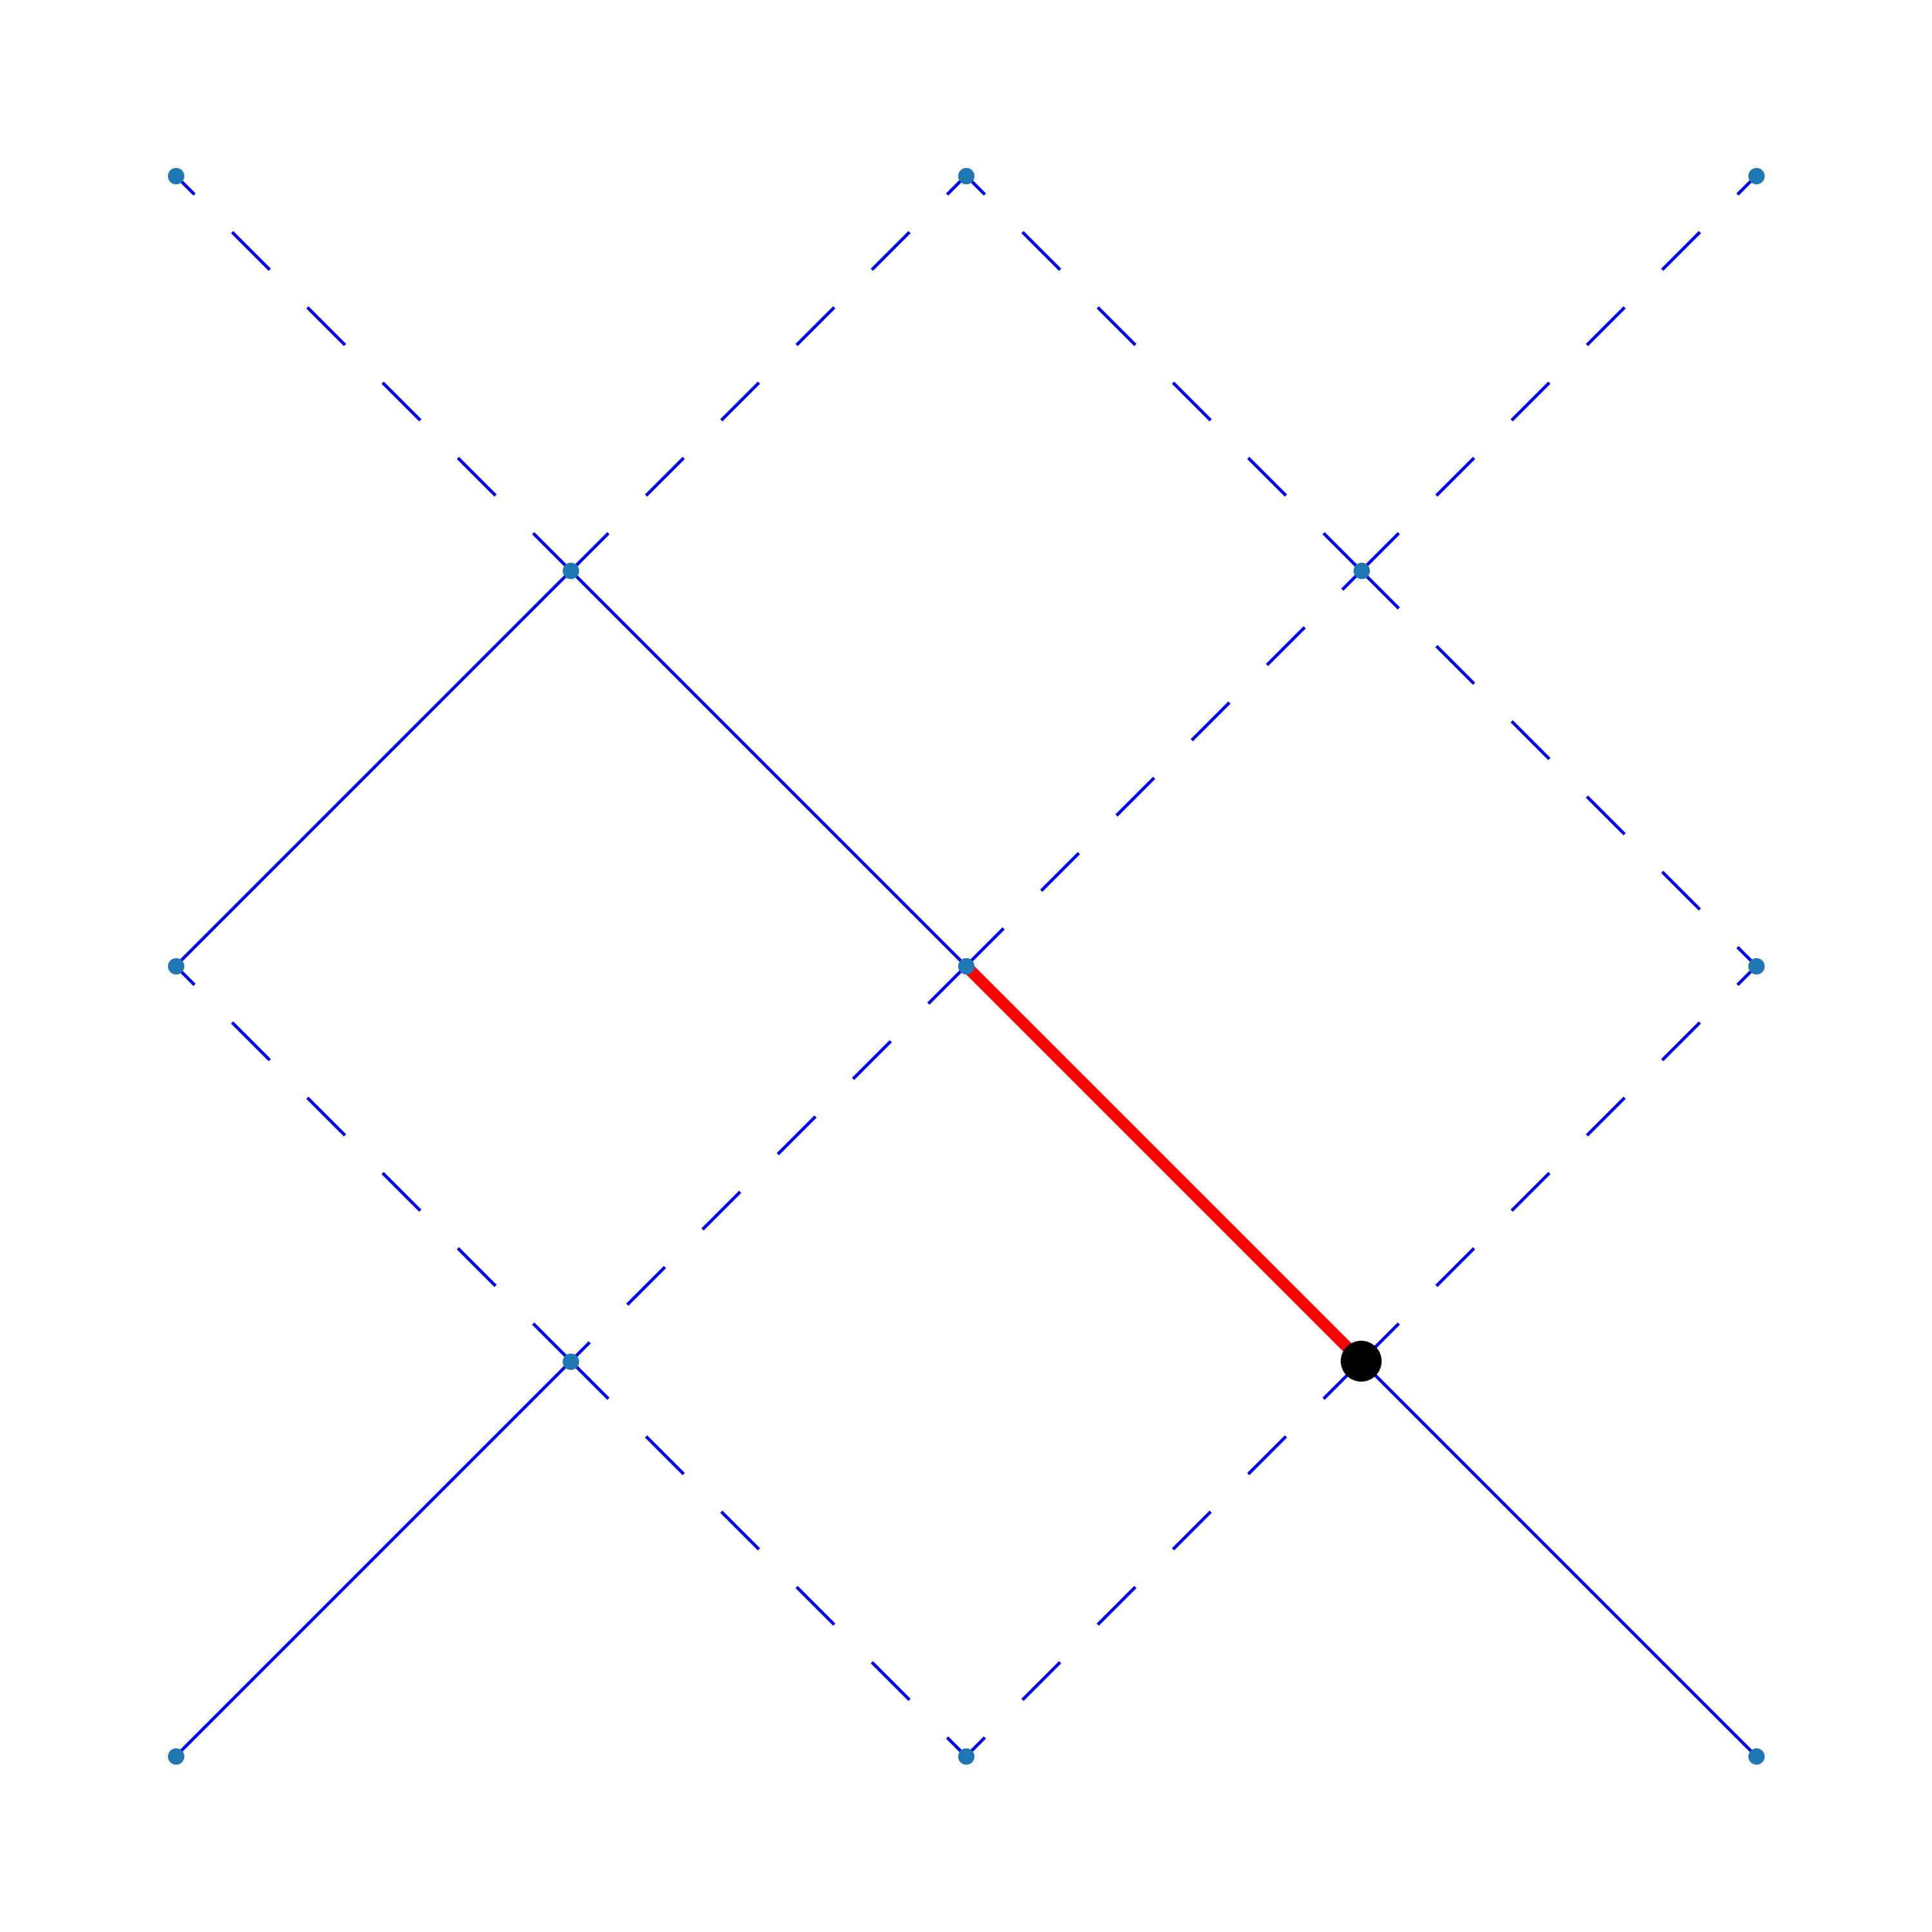
\includegraphics[width = 0.2\textwidth]{../images/game1/L5opit1p040.png}
            \caption{For Game 1, a realization of the payoff function for $p = 0.4$ (edges with a cost of 1 are represented by \protect\costOne and edges with 0 cost by \protect\costZero) along with the corresponding $1$-stage game (in red) starting from 0. The token is the black dot.}
        \end{figure}

    	Let $p$ be fixed, $\omega \in \Omega$ also, and consider a token placed at a given initial state $z \in \Z_r^2$. The game proceeds as follows: At each stage $m \in \N_+$, player 1 chooses top or bottom, then, knowing player 1's action, player 2 chooses left or right. The token then moves from its current state to the next, according to the combination of both actions: top-right, top-left, bottom-right or bottom-left. Player 1 then pays player 2 the cost associated with the corresponding edge. Thus, player 1 aims to minimize the payoff, while player 2 aims to maximize it.
        
        For $m \in \N_+$, we denote by $e_1, e_2, \ldots, e_m$ the path formed by the edges traversed in the game up to stage $m$. Since players can move the token in any of the four directions, the game is non-oriented; the path can loop back, intersect itself, and even form an infinite loop.

        A strategy for player 1 is a collection of mappings $(\sigma_m)_{m \geq 1}$, where each $\sigma_m$ assigns an action from the set $I$ to every possible history $(z, e_1, e_2, \ldots, e_m)$. For player 2, the strategy is the collection of mappings $(\tau_m)_{m \geq 1}$, where each $\tau_m$  assigns an action in the set $J$ to every possible sequence $(z, e_1, e_2, \ldots, e_m, i_m)$.

        For the $n$-stage game, the total payoff and value are
        \[
        	\gamma_n(z, \sigma, \tau) := \frac{1}{n}\sum_{m = 1}^{n}c(e_m) \; \text{ and } \; v_n(z) := \min_{\sigma \in \Sigma}\max_{\tau \in T} \gamma_n(z, \sigma, \tau) = \max_{\tau \in T}\min_{\sigma \in \Sigma} \gamma_n(z, \sigma, \tau).
        \]

        The total payoff of the game is defined as the limit superior of the average payoff:
        \[
        	\gamma(z, \sigma, \tau) := \limsup_{n \to \infty}\frac{1}{n}\sum_{m = 1}^{n}c(e_m).
        \]
        
        \begin{remark}
            In this context, the limit superior criterion is used to aggregate the payoff because it always exists within $\bar{\R}$, ensuring that it is a well-defined mathematical object. In contrast, the standard limit may not always exist. By using the $\limsup$ criterion, the outcome of the game is interpreted as the biggest possible long-term mean payoff achievable. In our scenario, where player 1 aims to minimize (and player 2 aims to maximize), this choice could be seen as disadvantageous for player 1 (and advantageous for player 2).
            %The choice between $\limsup$ and $\liminf$ is largely a matter of preference and should be guided by the needs of the specific model being analyzed. 
        \end{remark}

        Defined in this way, by Martin's theorem \cite{Martin1998}, the game has a value, which is
        \[
            v_p(z) := \min_{\sigma \in \Sigma}\max_{\tau \in T} \gamma(z, \sigma, \tau) = \max_{\tau \in T}\min_{\sigma \in \Sigma} \gamma(z, \sigma, \tau).
        \]

        Can we say something about $v_p(z)$? Does it depends on $z$? Is it random? Regarding these questions, we have the following result, presented by Ziliotto in \cite{Ziliotto2023}.

        \begin{theorem}\label{theorem-vz-independent-z-game1}
            $v_p(z)$ is independent of $z$ and is almost surely deterministic. 
        \end{theorem}

        The proof of this result primarily relies on game-theoretic arguments, which involves analyzing paths generated by both optimal and suboptimal strategies. Subsequently, a 0-1 law argument establishes that $v_p$ is deterministic. This will be further clarified in the next subsection, where we discuss the same result for the second game example.

        In the sequel, the limit value will be denoted simply by $v_p$.

        \begin{remark}\label{remark_v_p_non_decreasing}
           Note that the function $p \mapsto v_p$ is non-decreasing. This follows from the result stating that the parametrized family of probability measures $\{\Pbb_p\}_{p \in [0, 1]}$ can be coupled in an increasing way (see, for example, Proposition 2.1. in \cite{DuminilCopin2018}). 
        \end{remark}

        Given that $v_p$ is constant (taking values in $[0, 1]$), a natural question is: how much is it? In his presentation, Ziliotto further proved that it equals 1 if and only if $p$ is greater or equal than the probability threshold of oriented bond percolation. 

        Let $V$ be the event: ``there exists an infinite, vertically oriented path composed of 1s''. We call these paths 1-vertical. According to percolation theory (Theorem 3.30 in \cite{Grimmett2018}), there exists a \emph{critical probability} $p_1 \in (0, 1)$, such that:
        \begin{equation}\label{percolation-probability-1-vertical}
                \quad \Pbb_p(V) = \begin{cases}
                                    1       & p > p_1,\\  
                                    0       & p < p_1.
                                \end{cases}
        \end{equation}
        The function $\Pbb_p(V)$ (as a function of $p$) is called \emph{percolation probability}. The result is:

        \begin{theorem} \label{theorem-v1-p1}
            The value $v_p$ is 1 if and only if $p \geq p_1$. 
        \end{theorem}

        Building on the ideas from his presentation, we provide a non-rigorous sketch of the proof for this theorem, as certain aspects are essential for analyzing the value in both game examples.

        Due to the significance in our analysis of lattice structures that confer strategic advantages to players, we provide the following definition:

        \begin{definition}\label{def-right-structure-game1}
            An infinite subgraph $C$ with vertex set $V$ and edge set $E$, of the lattice $\Z_r^2$ is said to be a winning structure for player 1 if, for all $z \in V$, there exists an $i \in I$ such that, for all $j \in J$, $z + q(i, j) \in V$ and $\{z, z + q(i, j)\} \in E$. Similarly, is said to be a winning structure for player 2 if, for all $z \in V$, there exists a $j\in J$ such that, for all $i \in I$, $z + q(i, j) \in V$ and $\{z, z + q(i, j)\}$ is in $E$.
        \end{definition}

        Intuitively, these structures correspond to paths in the lattice where one player can capture the other, meaning they can keep the token within the structure regardless of the other player's actions. Note that this definition is independent of the edge costs.

        \begin{figure}[!hbt]
            \centering
                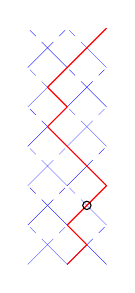
\begin{tikzpicture}[scale=0.5pt]
                    \def\a{0}; \def\b{5}; \def\aa{2}; \def\bb{3}

                    \foreach \x in {\aa, ..., \bb} {
                        \foreach \y in {\a, ..., \b} {
                            \draw[dashed, ultra thin, color = blue] (\x, \y) -- (\x + 0.5, \y + 0.5);
                            \draw[ultra thin, color = blue] (\x, \y) -- (\x + 0.5, \y - 0.5);
                            \draw[dashed, ultra thin, color = blue] (\x, \y) -- (\x - 0.5, \y + 0.5);
                            \draw[ultra thin, color = blue] (\x, \y) -- (\x - 0.5, \y - 0.5);
                        }
                    }

                    \def\xx{2.5}; \def\yy{-0.5}; \def\ur{0.5}; \def\dl{-0.5}
                    \draw[color = red] (\xx, \yy) -- (\xx + \ur, \yy + \ur);
                    \draw[color = red] (\xx + \ur, \yy + \ur) -- (\xx + \ur + \dl, \yy + 2*\ur);
                    \draw[color = red] (\xx + \ur + \dl, \yy + 2*\ur) -- (\xx + 3*\ur + \dl, \yy + 4*\ur);
                    \draw[color = red] (\xx + 3*\ur + \dl, \yy + 4*\ur) -- (\xx + 3*\ur + 2*\dl, \yy + 5*\ur);
                    \draw[color = red] (\xx + 3*\ur + 2*\dl, \yy + 5*\ur) -- (\xx + 3*\ur + 4*\dl, \yy + 7*\ur);
                    \draw[color = red] (\xx + 3*\ur + 4*\dl, \yy + 7*\ur) -- (\xx + 4*\ur + 4*\dl, \yy + 8*\ur);
                    \draw[color = red] (\xx + 4*\ur + 4*\dl, \yy + 8*\ur) -- (\xx + 4*\ur + 5*\dl, \yy + 9*\ur);
                    \draw[color = red] (\xx + 4*\ur + 5*\dl, \yy + 9*\ur) -- (\xx + 7*\ur + 5*\dl, \yy + 12*\ur);

                    \draw[color=black] (3., 1.) circle (3pt); 
                \end{tikzpicture}
                \caption{In red, a winning structure for player 2 in Game 1. If the state is at 
                    \protect\tikz[baseline, yshift=-2ex, scale=0.5pt] \protect\draw[color=black] (3., 1.) circle (3pt); 
                    and player 1 plays top, then player 2 will respond with right. Conversely, if player 1 plays bottom, player 2 will respond with left. A similar analysis can be done to any other vertex of the red path.}

                % At the point immediately preceding this one in the black path, player 2 will play $\shortarrow{0}$ regardless of player 1's action. 
                \label{figure-1-vertical}
        \end{figure} 

        Assume $p > p_1$. By \eqref{percolation-probability-1-vertical} and the corresponding reference, there exists a 1-vertical path with probability 1. Since this path is a winning structure for player 2 (see Figure \ref{figure-1-vertical}) and all edge costs along it are equal to 1, player 2 guarantees a value of 1. This proves that $v_p =  1$ in the supercritical regime. 

        The critical regime $p = p_1$ is more delicate. A 1-vertical path is no longer present. However, even in the absence of a 1-vertical path, it is still possible to devise a strategy for player 2 that moves through vertical oriented paths filled with 1s of increasing lengths, in such a way that he ensures a value of 1. To achieve this, the following result from Duminil-Copin et al. \cite{DuminilCopin18} is crucial. 
        % It provides an estimate on the probability of being within a distance $O(n)$ of a vertically oriented path filled with 1s of length $n$.

        \begin{proposition}\label{duminil-copin}
            There exists $\beta > 0$ such that for all $n$, the probability that there exists a vertically oriented path filled with 1s, of length greater than or equal to $n$, with its center at a distance less than or equal to $n^{1-\beta}$, is at least $1 - \exp(-n^{\beta})$. 
        \end{proposition} 
        
        For the $\beta$ of Proposition \ref{duminil-copin}, let $V_n$ be the event: ``there exists a vertically oriented path, with length greater than or equal to $n$ and composed of 1s, such that its center is at a distance less than or equal to $n^{1-\beta}$''. We denote by $1_n$-vertical a vertically oriented path of length at least $n$. 

        This proposition intuitively states that a $1_n$-vertical path with $n$ large enough occurs with high probability, in such a way that if you want to reach it, you don't have to wait too long. For player 2, reaching a $1_n$-vertical path may require sacrificing $n^{1-\beta}$ times 1, but this number is sublinear compared to the linear number of 1s that he will gain in the $1_n$-vertical path. 

        Based on this, for $n$ large enough, player 2 should aim to reach a $1_n$-vertical path and then stay in it for as long as possible. This approach is referred to as the $n$-strategy of player 2. If player 2 is smart he will stay for $n$ stages, but thereafter, he will not start with $n$ again. Instead, he will look for a path of length greater or equal than $n+1$, then greater or equal than $n+2$, and so on. 

        Let $N \geq 1$. At the stage $n \geq N$, the strategy for player 2 is: 
        \begin{itemize}
            \item[--] Play the $n$-strategy until leaving the path.
            \item[--] Then, search a $1_{n + 1}$-vertical path.
        \end{itemize}

        With this strategy, the only negative outcome to player 2 would be failing to find a sequence of paths $(1_n\text{-vertical})_{n \geq N}$. However, the probability of finding this sequence is given by
        \begin{eqnarray} \notag
            \Pbb_p\left(\bigcap_{n \geq N}V_n\right) & = & 1 - \Pbb_p\left(\exists n \geq N : V_n \text{ does not happen}\right) \\ \notag
            & \geq & 1 - \sum_{n \geq N} \Pbb_p(V_n^c)  \geq 1 - \sum_{n \geq N} \exp(-n^{\beta}), 
        \end{eqnarray}
        % \begin{eqnarray} \notag
        %     \Pbb_p\left(\bigcap_{n \geq N}V_n\right) & = & 1 - \Pbb_p\left(\exists n \geq N : V_n \text{ does not happen}\right) \\ \notag
        %     & \geq & 1 - \sum_{n \geq N} \Pbb_p(V_n^c) \\ \notag
        %     & \geq & 1 - \sum_{n \geq N} \exp(-n^{\beta}), 
        % \end{eqnarray}
        where the first inequality follows from the union bound, and the final result comes from Proposition \ref{duminil-copin}, which states that $\Pbb_p(V_n) > 1 - \exp(-n^{\beta})$. As $N$ tends to infinity, this probability tends to 1. 

        From this, it follows that with positive probability, player 2 can guarantee a value of 1. Therefore, with positive probability, the value is 1. Since $v_p$ is deterministic, it follows that $v_p =  1$. 

        Avelio Sepúlveda and Bruno Ziliotto are currently working on a paper that addresses the link between this game and oriented bond percolation in $\Z^2$. In the subcritical regime, they have demonstrated that player 1 guarantees a value strictly smaller than 1, thereby completing the proof of Theorem \ref{theorem-v1-p1}. They achieve this by considering a strategy for player 1 in which he always plays top, and by showing that the path followed by the token under this strategy has a positive density of 0s because it is oriented. They also established that the map $p \mapsto v_p$ is continuous at $p_1$. 

        Additionally, they have a result indicating that for $p$ sufficiently small, player 1 can achieve a value of 0. This result cannot be inferred from the previous analysis due to the lack of symmetry in the game. In the following, we outline our approach to better understand the conditions under which the value is 0.

        We start by identifying the winning structures for player 1. To do this, we examine all possible local configurations around a vertex. This approach yields a geometric characterization of such structures.

        First, why are infinite vertically oriented paths the winning structures for player 2? Geometrically, it is easily observed that in a winning structure for player 2, locally around each vertex, the edges must take one of the following four configurations (see Figure \ref{figure-1-vertical}):

        \begin{center}
            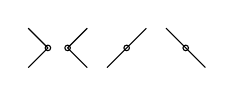
\begin{tikzpicture}[scale=0.5pt] 
                \draw[color=black!100] (-0.5, 0) circle (2pt);
                \draw[color = black!100] (-1., -0.5) -- (-0.5, 0);
                \draw[color = black!100] (-0.5, 0) -- (-1., 0.5);

                \draw[color=black!100] (0, 0) circle (2pt); 
                \draw[color = black!100] (0.5,-0.5) -- (0, 0);
                \draw[color = black!100] (0, 0) -- (0.5, 0.5);

                \draw[color=black!100] (1.5, 0) circle (2pt);
                \draw[color = black!100] (1, -0.5) -- (2, 0.5);

                \draw[color=black!100] (3, 0) circle (2pt);
                \draw[color = black!100] (2.5, 0.5) -- (3.5, -0.5);
            \end{tikzpicture}
        \end{center}
       \noindent Configurations that do not guarantee this are:
            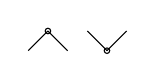
\begin{tikzpicture}[scale=0.5pt] 
                \draw[color=black!100] (-1., -1) circle (2pt);
                \draw[color = black!100] (-1.5, -1.5) -- (-1, -1);
                \draw[color = black!100] (-0.5, -1.5) -- (-1, -1);

                \draw[color=black!100] (0.5, -1.5) circle (2pt); 
                \draw[color = black!100] (0, -1) -- (0.5, -1.5);
                \draw[color = black!100] (0.5, -1.5) -- (1, -1);
            \end{tikzpicture},
            where player 1 always has an option to escape from the path. This confirms the verticality of the structure. In contrast, structures with these local forms are controlled by player 1 and we state this as a proposition.

       \begin{proposition} \label{rigtht-structure-player1-game1}
        An infinite subgraph $C \subset \Z^2$ is a winning structure for player 1 if around each vertex one of the following local configurations is present: 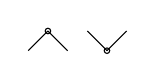
\begin{tikzpicture}[scale=0.5pt] 
                \draw[color=black!100] (-1., -1) circle (2pt);
                \draw[color = black!100] (-1.5, -1.5) -- (-1, -1);
                \draw[color = black!100] (-0.5, -1.5) -- (-1, -1);

                \draw[color=black!100] (0.5, -1.5) circle (2pt); 
                \draw[color = black!100] (0, -1) -- (0.5, -1.5);
                \draw[color = black!100] (0.5, -1.5) -- (1, -1);
            \end{tikzpicture}

            % \begin{figure}[!hbt]
            %     \centering
            %     \begin{tikzpicture}[scale=0.5pt] 
            %         \fill[color=black!100] (-1., 0) circle (1pt);
            %         \draw[color = black!100] (-1.5, -0.5) -- (-1, 0);
            %         \draw[color = black!100] (-0.5, -0.5) -- (-1, 0);

            %         \fill[color=black!100] (0, 0) circle (1pt); 
            %         \draw[color = black!100] (-0.5, 0.5) -- (0, 0);
            %         \draw[color = black!100] (0.5, 0.5) -- (0, 0);

            %         % \fill[color=black!100] (3, 0) circle (1pt);
            %         % \draw[color = black!100] (3, 0) -- (3 - 0.5, 0 + 0.5);
            %         % \draw[color = black!100] (3, 0) -- (3 + 0.5, 0 + 0.5);
            %         % \draw[color = black!100] (3, 0) -- (3 + 0.5, 0 - 0.5);

            %         % \fill[color=black!100] (1.5, 0) circle (1pt);
            %         % \draw[color = black!100] (1.5, 0) -- (1.5 - 0.5, 0 + 0.5);
            %         % \draw[color = black!100] (1.5, 0) -- (1.5 + 0.5, 0 + 0.5);
            %         % \draw[color = black!100] (1.5, 0) -- (1.5 - 0.5, 0 - 0.5);

            %         % \fill[color=black!100] (4.5, 0) circle (1pt); 
            %         % \draw[color = black!100] (4.5, 0) -- (4.5 - 0.5, 0 - 0.5);
            %         % \draw[color = black!100] (4.5, 0) -- (4.5 - 0.5, 0 + 0.5);
            %         % \draw[color = black!100] (4.5, 0) -- (4.5 + 0.5, 0 - 0.5);

            %         % \fill[color=black!100] (6, 0) circle (1pt); 
            %         % \draw[color = black!100] (6, 0) -- (6 - 0.5, 0 - 0.5);
            %         % \draw[color = black!100] (6, 0) -- (6 + 0.5, 0 + 0.5);
            %         % \draw[color = black!100] (6, 0) -- (6 + 0.5, 0 - 0.5);
            %     \end{tikzpicture}
            % \end{figure}
       \end{proposition}

       A finite portion of these structures could take on a seemingly intricate form:

       \begin{center}
    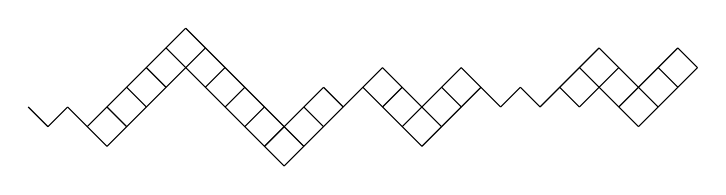
\begin{tikzpicture}[scale=0.5pt]
    \def\a{-5.5}
    \def\b{10.5}

    \draw[color = black!100] (0, 0.5) -- (1.5, 2);
    \draw[color = black!100] (0.5, 0) -- (3, 2.5);
    \draw[color = black!100] (3, 1.5) -- (3.5, 2);
    \draw[color = black!100] (3.5, 1) -- (5, 2.5);
    \draw[color = black!100] (4, 0.5) -- (5.5, 2);
    \draw[color = black!100] (6, 1.5) -- (6.5, 2);
    \draw[color = black!100] (7, 1.5) -- (8.5, 3);
    \draw[color = black!100] (8, 1.5) -- (9, 2.5);
    \draw[color = black!100] (9, 1.5) -- (9.5, 2);
    \draw[color = black!100] (9.5, 1) -- (10, 1.5);

    \draw[color = black!100] (-2, 2.5) -- (0.5, 0);
    \draw[color = black!100] (-2, 3.5) -- (1, 0.5);
    \draw[color = black!100] (1, 1.5) -- (1.5, 1);
    \draw[color = black!100] (1.5, 2) -- (2, 1.5);
    \draw[color = black!100] (2.5, 2) -- (4, 0.5);
    \draw[color = black!100] (3, 2.5) -- (4.5, 1);
    \draw[color = black!100] (4.5, 2) -- (5, 1.5);
    \draw[color = black!100] (5, 2.5) -- (6, 1.5);
    \draw[color = black!100] (6.5, 2) -- (7, 1.5);
    \draw[color = black!100] (7.5, 2) -- (8, 1.5);
    \draw[color = black!100] (8, 2.5) -- (9.5, 1);
    \draw[color = black!100] (8.5, 3) -- (10, 1.5);
    \draw[color = black!100] (11, 2.5) -- (10, 1.5);
    \draw[color = black!100] (10.5, 3) -- (9.5, 2);

    \draw[color = black!100] (10, 2.5) -- (10.5, 2);
    \draw[color = black!100] (10.5, 3) -- (11, 2.5);

    \draw[color = black!100] (-2, 2.5) -- (-4, 0.5);
    \draw[color = black!100] (-2, 3.5) -- (-4.5, 1);
    \draw[color = black!100] (-3.5, 1.0) -- (-4, 1.5);
    \draw[color = black!100] (-3, 1.5) -- (-3.5, 2);
    \draw[color = black!100] (-2.5, 2.0) -- (-3, 2.5);
    \draw[color = black!100] (-2, 2.5) -- (-2.5, 3);

    \draw[color = black!100] (-2, 2.5) -- (-1.5, 3);
    \draw[color = black!100] (-1.5, 2) -- (-1.0, 2.5);
    \draw[color = black!100] (-1, 1.5) -- (-0.5, 2);
    \draw[color = black!100] (-0.5, 1) -- (0, 1.5);
    \draw[color = black!100] (0, 0.5) -- (0.5, 1);

    \draw[color = black!100] (-5, 1.5) -- (-4, 0.5);
    \draw[color = black!100] (-5, 1.5) -- (-5.5, 1.);
    \draw[color = black!100] (-6, 1.5) -- (-5.5, 1.0);

    % \coordinate (A) at (11.3, 2.5);
    % \coordinate (B) at (11.6, 2.5);
    % \coordinate (C) at (11.9, 2.5);
    
    % % Draw the dots
    % \fill (A) circle (1pt);
    % \fill (B) circle (1pt);
    % \fill (C) circle (1pt);

    % \coordinate (A) at (-6.3, 1.5);
    % \coordinate (B) at (-6.6, 1.5);
    % \coordinate (C) at (-6.9, 1.5);
    
    % % Draw the dots
    % \fill (A) circle (1pt);
    % \fill (B) circle (1pt);
    % \fill (C) circle (1pt);

    \end{tikzpicture}
\end{center}

       In the following, we refer to winning structures for player 1 that are filled with $0$s, as $0$-horizontal structures, and denote the event: ``there exists a $0$-horizontal structure'' by $H_0$. The percolation probability for these structures is $\Pbb_p(H_0)$ and the critical probability $p_0$ is defined as
        \[
            p_0 := \sup\{ p \in [0, 1] : \Pbb_p(H_0) = 1\}.
        \]     

        \begin{theorem}\label{conjecture-v0-p0}
            For all $p < p_0$, $v_p = 0$.
        \end{theorem}
        
        \begin{proof}
            If $p < p_0$, a $0$-horizontal structure appears. Player 1 can reach such a structure in a finite number of stages. Since this structure is a winning one for player 1, it guarantees a value of $0$. Therefore, $v_p =  0$.

        \end{proof}

        Is fundamental to establish that $0 < p_0 < 1$. We state this as a theorem:

        \begin{theorem}\label{theorem-p_0}
            $0 < p_0 < 1$.
        \end{theorem}

        % We could not find any references or studies addressing percolation for these types of structures; therefore, we provide a proof for this result.

        \begin{proof}
           Let denote by $A$ the event: ``there exists a 0-horizontal structure composed entirely by squares'', and let $B$ be the event: ``there exists an horizontally oriented path filled with 0s''. We have the following relation between these events and $H_0$:
           \begin{equation}\label{A-H_0-B}
                A \subset H_0 \subset B.
           \end{equation}

           The inclusion $A \subset H_0$ is because any 0-horizontal structure composed entirely of squares is itself a 0-horizontal structure. The inclusion $H_0 \subset B$ is more subtle; it follows from the geometric local characterization of the vertices in a 0-horizontal structure. To see why this is the case, imagine traversing a 0-horizontal structure from left to right. At each vertex, you have one of the two possibilities: moving top-right 
           \begin{tikzpicture}[scale=0.5pt] 
                \draw[color=black!100] (0.5, -1.5) circle (2pt); 
                \draw[color = black!100] (0.5, -1.5) -- (1, -1);
            \end{tikzpicture}, or moving bottom-right 
           \begin{tikzpicture}[scale=0.5pt] 
                \draw[color=black!100] (-1., -1) circle (2pt);
                \draw[color = black!100] (-0.5, -1.5) -- (-1, -1);
           \end{tikzpicture}. By consistently choosing one of these options at each vertex, you will end up with an infinite, horizontally oriented path filled with 0s.

           As mentioned earlier (see \eqref{percolation-probability-1-vertical}), percolation theory tells us that the critical probability for $B$ is $1 - p_1 < 1$. Therefore, using the second relation in \eqref{A-H_0-B}, we obtain $p_0 \leq 1-p_1 < 1$. 

           It remains to be shown that $p_0 > 0$. 

           Define the critical probability of the event $A$ as 
           $$
                p^* := \sup\{p \in [0, 1] : \Pbb_p(A) = 1\}.
           $$ 
           From the first relation in \eqref{A-H_0-B}, we have $p^* < p_0$. Thus, it suffices to prove that $p^* > 0$. 

           To do this, we use a Peierls-type argument. This argument focuses on contour-like structures or boundaries between regions with different configurations. In percolation theory, a key component is the use of the \emph{dual} lattice to analyze these boundaries; contours in the original lattice can be mapped onto paths or circuits in the dual lattice..

            % The Peierls argument, originally developed by physicist Rudolf Peierls for the 2D Ising model, is a powerful technique in statistical mechanics and percolation theory for establishing bounds on critical parameters and demonstrating the existence of phase transitions, particularly in low-dimensional systems. This argument focuses on contour-like structures or boundaries between regions with different configurations. A key component is the use of the \emph{dual} lattice to analyze these boundaries; contours in the original lattice can be mapped onto paths or circuits in the dual lattice. This approach can simplify complex random geometric problems into more manageable combinatorial ones.
            % It demonstrates that below a certain critical temperature or probability, the system transitions from a disordered phase to an ordered one, or in percolation theory, from small clusters to the formation of an infinite cluster.
            % The Peierls argument has been adapted and generalized for various models and dimensions, making it a versatile tool for understanding phase transitions across different systems.

            Consider the dual lattice $\tilde{\mathbb{Z}}_r^2$, which is a copy of our original square lattice translated by the vector $(0, 1/2)$. Define a 1-1 mapping where $e \in \E_r^2$ and $\tilde{e} \in \tilde{\mathbb{E}}_r^2$ are said to be \emph{dual to each other} if $\tilde{e}$ crosses $e$. Using the original random variables $\{c(e)\}_{e \in \E_r^2}$, we define random variables for the dual edges $\{\tilde{c}(\tilde{e})\}_{\tilde{e} \in \tilde{\mathbb{E}}_r^2}$ by setting $\tilde{c}(\tilde{e}) = 1 - c(e)$. Note that the distribution of $\tilde{c}$ is a translation by $(0, 1/2)$ of the distribution $\Pbb_{1-p}$.
 
            In what follows, we refer to a 0-square as a square with all its edges equal to 0. The length of a structure will be understood as the number of squares it contains and the distance between two squares is understood as the distance between their centers.
            
            If there is no 0-horizontal structure composed entirely of 0-squares, then the origin cannot be contained within one. From the duality relation, it follows that if there is no 0-horizontal structure composed entirely of 0-squares containing the origin, there must exist an $n \in \N_+$ such that the square $[-n, n] \times [-n, n]$ is crossed vertically by a dual path that does not contain 0-squares. A dual path can be interpreted as another different structure. 

           From all this, using the union bound, Markov inequality and the fact that a dual path from $[-n, n] \times \{n\}$ to $[-n, n] \times \{-n\}$ must have at least $2n$ edges, we obtain
           \begin{eqnarray} \notag
                \Pbb_p(A^c) & \leq & \sum_{n \geq 1} \Pbb_p\left(\substack{\text{there exist a dual path that does not contain} \\ \text{0-squares, from } [-n, n] \times \{n\} \text{ to } [-n, n] \times \{-n\}}\right) \\ \notag
                            & \leq & \sum_{n \geq 1} \E_p\left(\substack{\text{number of dual paths that does not contain} \\ \text{0-squares, from } [-n, n] \times \{n\} \text{ to } [-n, n] \times \{-n\}}\right) \\ \notag
                            & \leq & \sum_{n \geq 1} \sum_{l \geq 2n} \kappa(l) \Pbb_p\left(\substack{\text{all squares of a given dual path} \\ \text{of length $l$ are not  0-squares}}\right),
           \end{eqnarray}   
           where $\kappa(l) = \#\{\text{of dual paths from } [-n, n] \times \{-n\} \text{ to } [-n, n] \times \{n\} \text{ of length } l\}$.

           Let each square (of any of the lattices considered) be associated with its center, and define the center of a square to be open if and only if the square is a 0-square. With this definition, the problem of finding a path in this percolation setting --where paths are composed of squares with edges that can be either open or closed-- translates into finding a path in a 1-dependent site percolation model. In this model, for any $k \geq 2$ and any sites $z_1, z_2, \ldots, z_k \in \Z^2$ that are at a distance of at least 2 (i.e., they are not immediate neighbors), the random variables indicating whether each site is open are independent.

           Let $\tilde{\alpha}$ be the given oriented dual path of length $l$. For any square in $\tilde{\alpha}$ at most 5 squares of $\tilde{\mathbb{Z}}^2$ are within a distance of 1 from it. Hence, there exists a sub-path $\tilde{\beta}$ of at least $l/5$ squares of $\tilde{\alpha}$ such that any two squares $x, y \in \tilde{\beta}$ are at a distance of at least $2$. Between these paths $\tilde{\alpha}$ and $\tilde{\beta}$ we have the following relation, 
           $$
                \Pbb_p(\text{every square in } \tilde{\alpha} \text{ is not a 0-square}) \leq \Pbb_p(\text{every square in } \tilde{\beta} \text{ is not a 0-square}).
           $$ 
           Moreover, since the costs of the squares of $\tilde{\beta}$ are independent, we get
           \[
                \Pbb_p(\text{every square in } \tilde{\alpha} \text{ is not a 0-square}) \leq (1 - (1-p)^4)^{|\tilde{\beta}|} \leq (1 - (1-p)^4)^{l/5}. 
           \]

           For $\kappa(l)$, the following upper bound can be given:
           \[
                \kappa(l) \leq (2n)^25^l,
           \]
           where $(2n)^2$ accounts for the number of possible starting and ending squares of the path, and $5^l$ represents the number of possible ways to complete the path, considering the choices for each square within a distance smaller than 2.

           Consequently, 
           \[
                \Pbb_p(A^c) \leq 4 \sum_{n \geq 1} n^2 \sum_{l \geq 2n} 5^l(1 - (1-p)^4))^{l/5} \to 0, \text{ as } p \to 0.
           \]
           Hence, by choosing $p$ small enough such that
           \[
                \Pbb_p(A^c) < 1,
           \]
           we obtain $\Pbb_p(A) > 0$. Since the event $A$ is translation invariant and $\Pbb_p$ is ergodic (see Lemma 2.8 in \cite{DuminilCopin2018}), its probability must be either 0 or 1. Therefore, for sufficiently small $p$, $\Pbb_p(A) = 1$, implying $p^* > 0$.

        \end{proof}
        
        % Let denote by $\Psi(p)$ the probability that there exists \text{some} winning structure for player 1, not necessarily containing the origin. Obviously $\Psi(p) \geq \psi(p)$ and thus $\Psi(p) > 0$ for $p > p_0$. One can show more. In fact, we have the following zero-one law $\Psi(p)$: 
        % \[
        %     \Psi(p) = \begin{cases}
        %                              0      & p < p_0, \\  
        %                              1      & p > p_0.
        %                \end{cases}
        % \]
        
        Note that the only winning structure for player 1 that does not include squares is the infinite concatenation of one of the two local configurations, specifically, the path:
        \begin{center}
            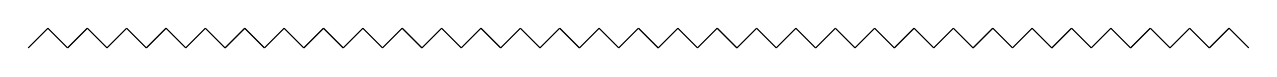
\begin{tikzpicture}[scale=0.5pt]
                \def\aa{-20}
                \def\bb{10}
                    \foreach \x in {\aa, ..., \bb} {
                        \draw[color = black!100] (\x, 0) -- (\x + 0.5, 0.5);
                        \draw[color = black!100] (\x + 0.5, 0.5) -- (\x + 1, 0.0);
                    }
            \end{tikzpicture}
        \end{center}

        \noindent However, the probability of having a path like this with $L$ edges and all edge costs equal 0 is $(1 - p)^L$. Therefore,
        \[
            \Pbb_p(\ldots 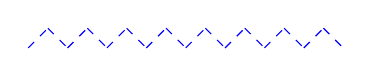
\begin{tikzpicture}[scale=0.5pt]
                    \def\aa{-5}
                    \def\bb{2}
                        \foreach \x in {\aa, ..., \bb} {
                            \draw[dashed, thin, color = blue] (\x, 0) -- (\x + 0.5, 0.5);
                            \draw[dashed, thin, color = blue] (\x + 0.5, 0.5) -- (\x + 1, 0.0);
                        }
                \end{tikzpicture} \ldots) = \lim_{L \to \infty} (1 - p)^L = \begin{cases}
                                                                            1   &   p = 0, \\
                                                                            0   &   p > 0. 
                                                                        \end{cases}
       \]
       This means that the critical probability threshold for this structure is 0, indicating that there is no phase transition for it. Aside from this case, all 0-horizontal structures strictly contain an infinite, horizontally oriented path (see the analysis used to prove the second inclusion in \eqref{A-H_0-B}). Therefore, the following result follows:

        \begin{proposition} \label{theorem-relation-p0-p1}
            $p_0 < 1-p_1$.
        \end{proposition}
 
        % \begin{eqnarray*}
        %     \Pbb_p(H_0) & = & \Pbb_p(H_0 \backslash \ldots \begin{tikzpicture}[scale=0.5pt]
        %                                         \def\aa{-5}
        %                                         \def\bb{2}
        %                                             \foreach \x in {\aa, ..., \bb} {
        %                                                 \draw[color = black!100] (\x, 0) -- (\x + 0.5, 0.5);
        %                                                 \draw[color = black!100] (\x + 0.5, 0.5) -- (\x + 1, 0.0);
        %                                             }
        %                                     \end{tikzpicture} \ldots) + \Pbb_p(\ldots 
        %                                     \begin{tikzpicture}[scale=0.5pt]
        %                                         \def\aa{-5}
        %                                         \def\bb{2}
        %                                             \foreach \x in {\aa, ..., \bb} {
        %                                                 \draw[color = black!100] (\x, 0) -- (\x + 0.5, 0.5);
        %                                                 \draw[color = black!100] (\x + 0.5, 0.5) -- (\x + 1, 0.0);
        %                                             }
        %                                     \end{tikzpicture} \ldots) \\
        %                 & < & \Pbb_{p, \rightarrow}(V_0 \backslash \ldots 
        %                                     \begin{tikzpicture}[scale=0.5pt]
        %                                         \def\aa{-5}
        %                                         \def\bb{2}
        %                                             \foreach \x in {\aa, ..., \bb} {
        %                                                 \draw[color = black!100] (\x, 0) -- (\x + 0.5, 0.5);
        %                                                 \draw[color = black!100] (\x + 0.5, 0.5) -- (\x + 1, 0.0);
        %                                             }
        %                                     \end{tikzpicture} \ldots) + \Pbb_p'(\ldots 
        %                                     \begin{tikzpicture}[scale=0.5pt]
        %                                         \def\aa{-5}
        %                                         \def\bb{2}
        %                                             \foreach \x in {\aa, ..., \bb} {
        %                                                 \draw[color = black!100] (\x, 0) -- (\x + 0.5, 0.5);
        %                                                 \draw[color = black!100] (\x + 0.5, 0.5) -- (\x + 1, 0.0);
        %                                             }
        %                                     \end{tikzpicture} \ldots)  \\
        %                 & < & \Pbb_p'(V_0)
        % \end{eqnarray*}  

        Motivated by Theorem \ref{theorem-v1-p1}, we propose the following conjecture:

        \begin{conjecture}\label{conjecture-v0-p0}
            The value $v_p$ is 0 if and only if $p \leq p_0$.
        \end{conjecture}

        For proving this result in the critical regime $p = p_0$, a result similar to Proposition \ref{duminil-copin} would be needed, but for 0-horizontal structures. However, we have not found any references to this type of structure in the literature, and proving this is not straightforward. Nevertheless, we would very much like to attempt this, so it remains a task for future work. Similarly, proving that if $p > p_0$, then $v_p > 0$ should be feasible --following the idea of Bruno and Avelio-- by considering a strategy for player 2 where he always plays right, regardless of player 1's actions, and then demonstrating that the path followed by the token under this strategy has a positive density of 1s. Thus, with this strategy, player 2 guarantees a value strictly greater than 0.

        In the following, we introduce the second percolation game, whose analysis similarly revolves on identifying the winning structures for each player.

    \subsection{Game 2}     
        This game has the same state space and action sets as the previous game, but without rotating the square lattice $\Z^2$. 

        At each stage $m \in \N_+$, there are 2 substages:
        \begin{itemize}
                \item[--] player 1 chooses an action $i_m$, and the state moves to $z_{m+1/2} = z_m + (0, i_m)$.
                \item[--] Then, knowing player 1's action, player 2 chooses an action $j_m$, and the token moves to $z_{m+1} = z_{m+1/2} + (j_m, 0) = z_m + (j_m, i_m)$.
        \end{itemize}
        The payoff for the $m$-stage game is given by $g_m^{\omega} := g_{\omega}(z_{m}, i_m, 0) + g_{\omega}(z_{m+1/2}, 0, j_m)$. Player 1 receives $g_m^{\omega}$ , while player 2 receives $-g_m^{\omega}$. Note that, unlike the previous game, the token moves twice at each stage. However, the transition function remains the same. This time, player 1 maximizes.

        \begin{figure}[H]
            \centering
            \includegraphics[width = 0.2\textwidth]{../images/game2/L5grid_arrowsit0p040.png}    
            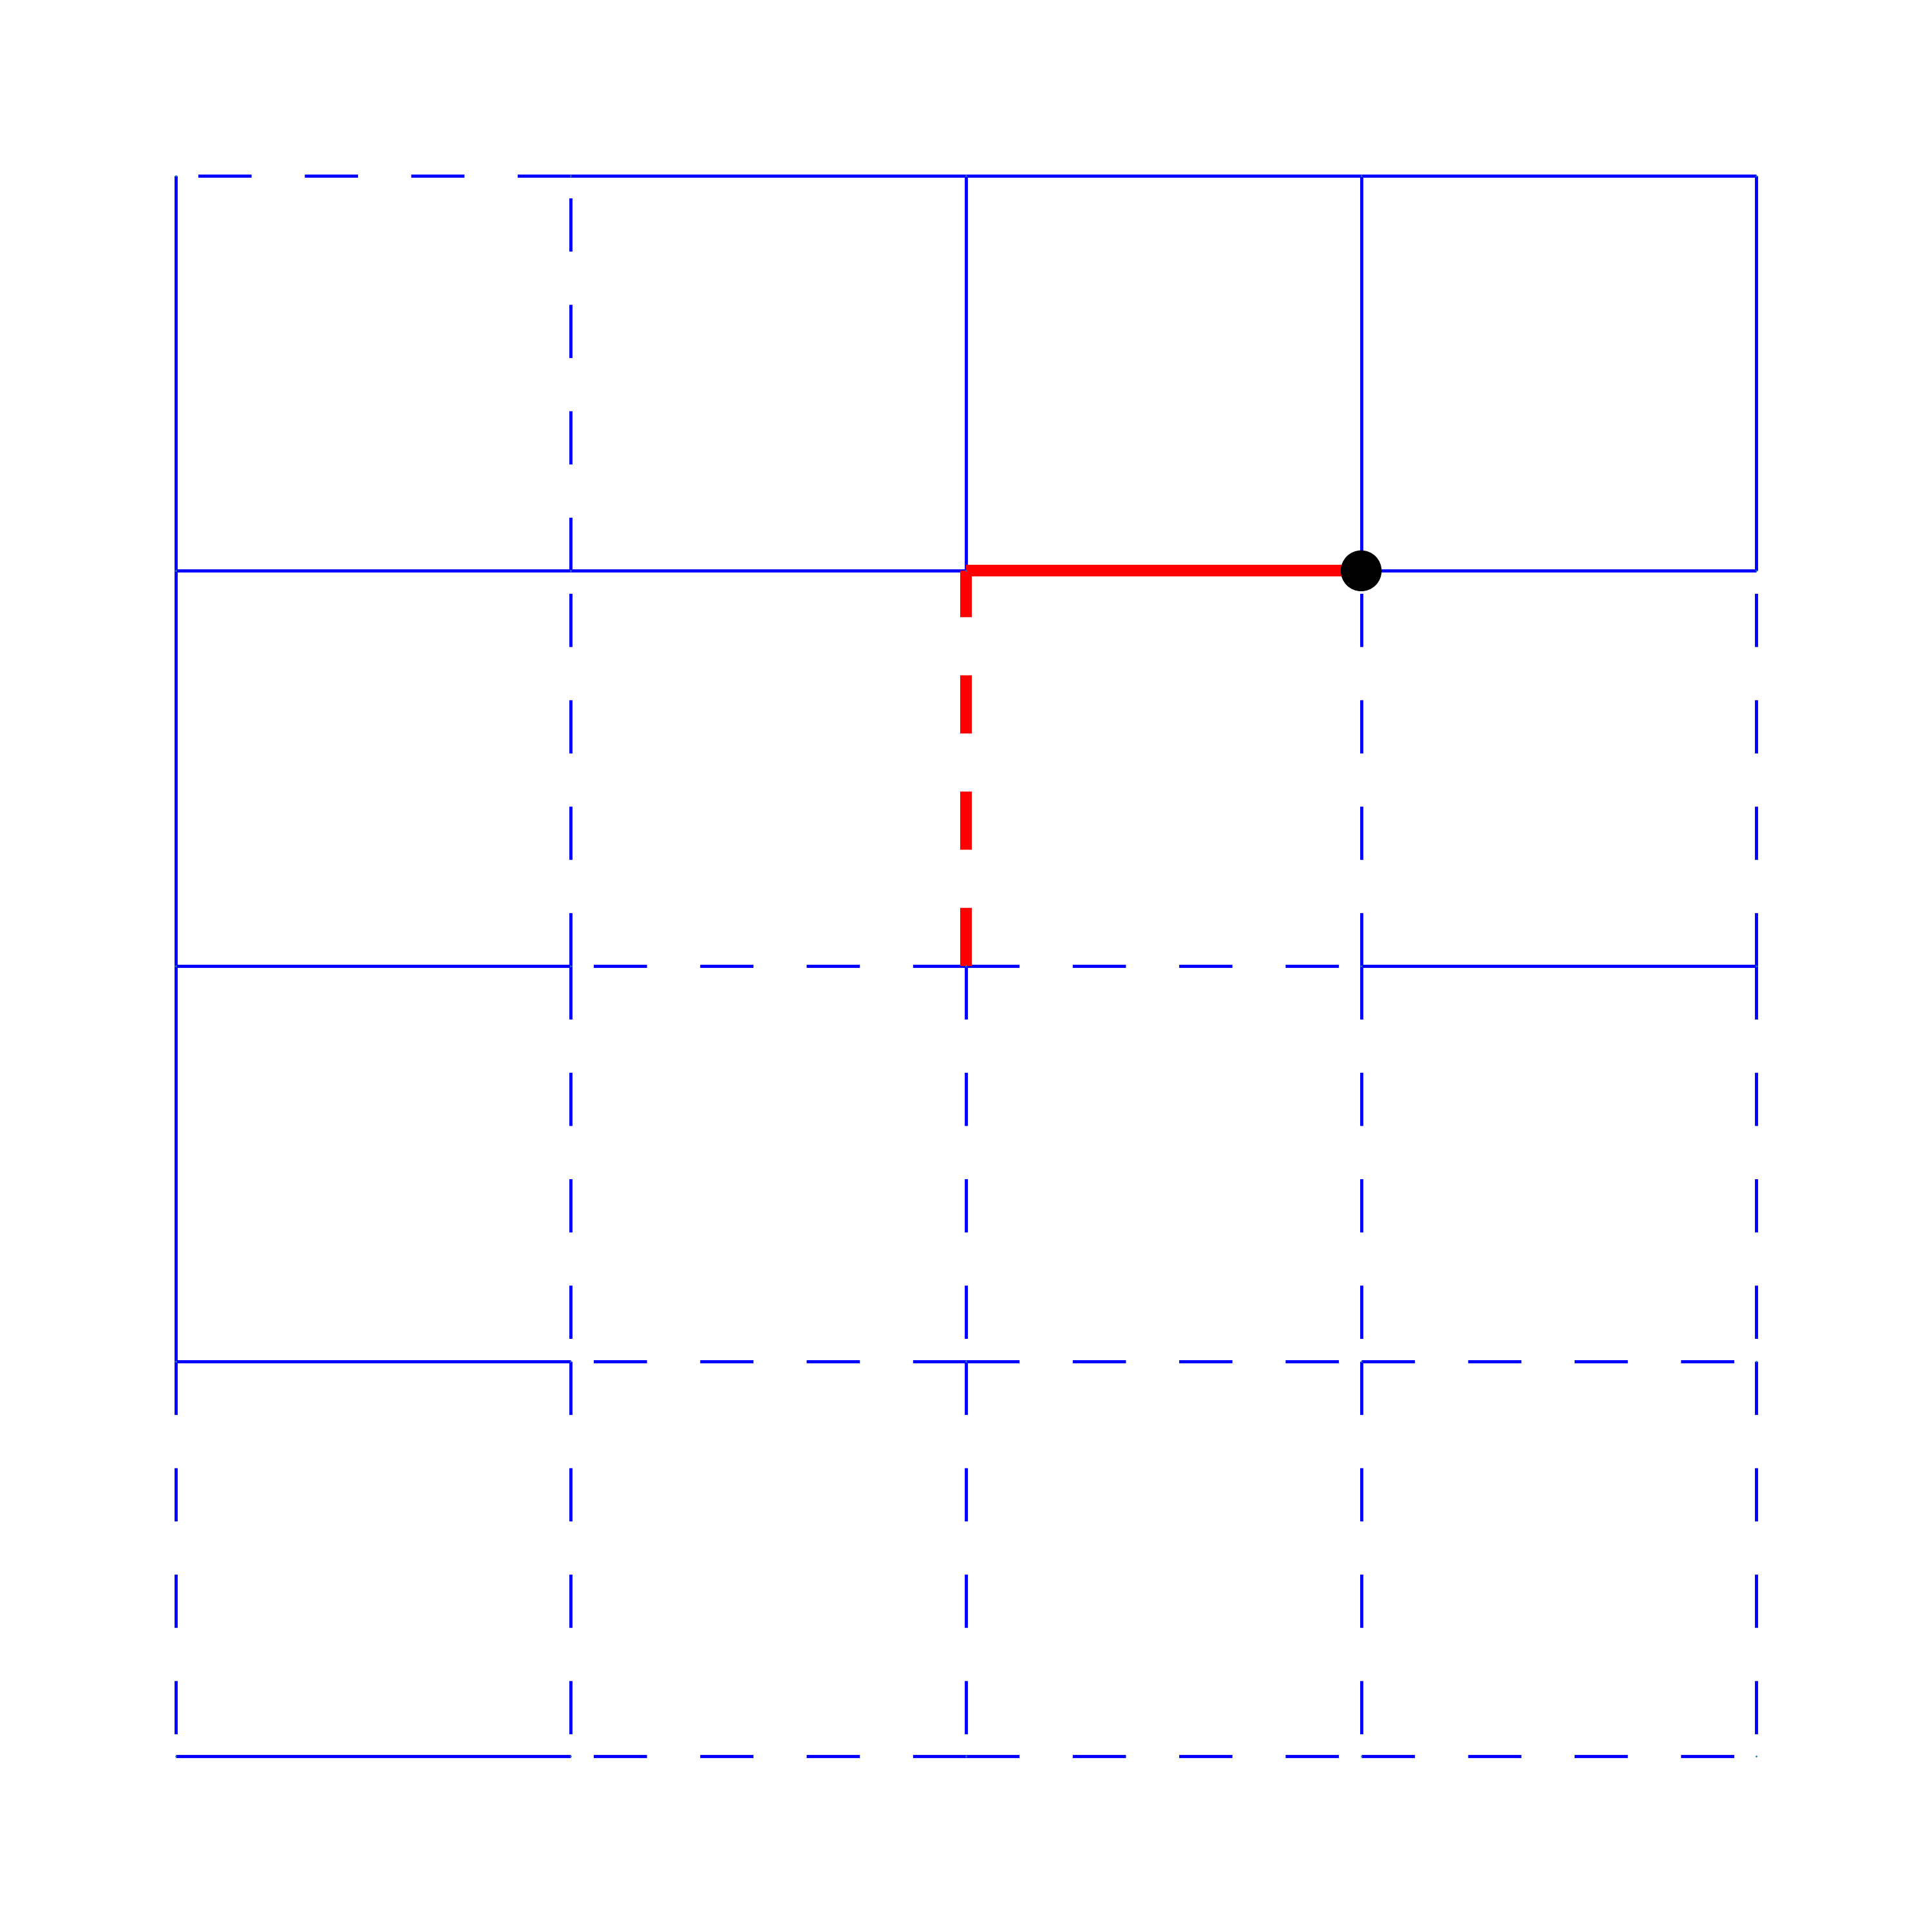
\includegraphics[width = 0.2\textwidth]{../images/game2/Ll1opit1p040.png}            
            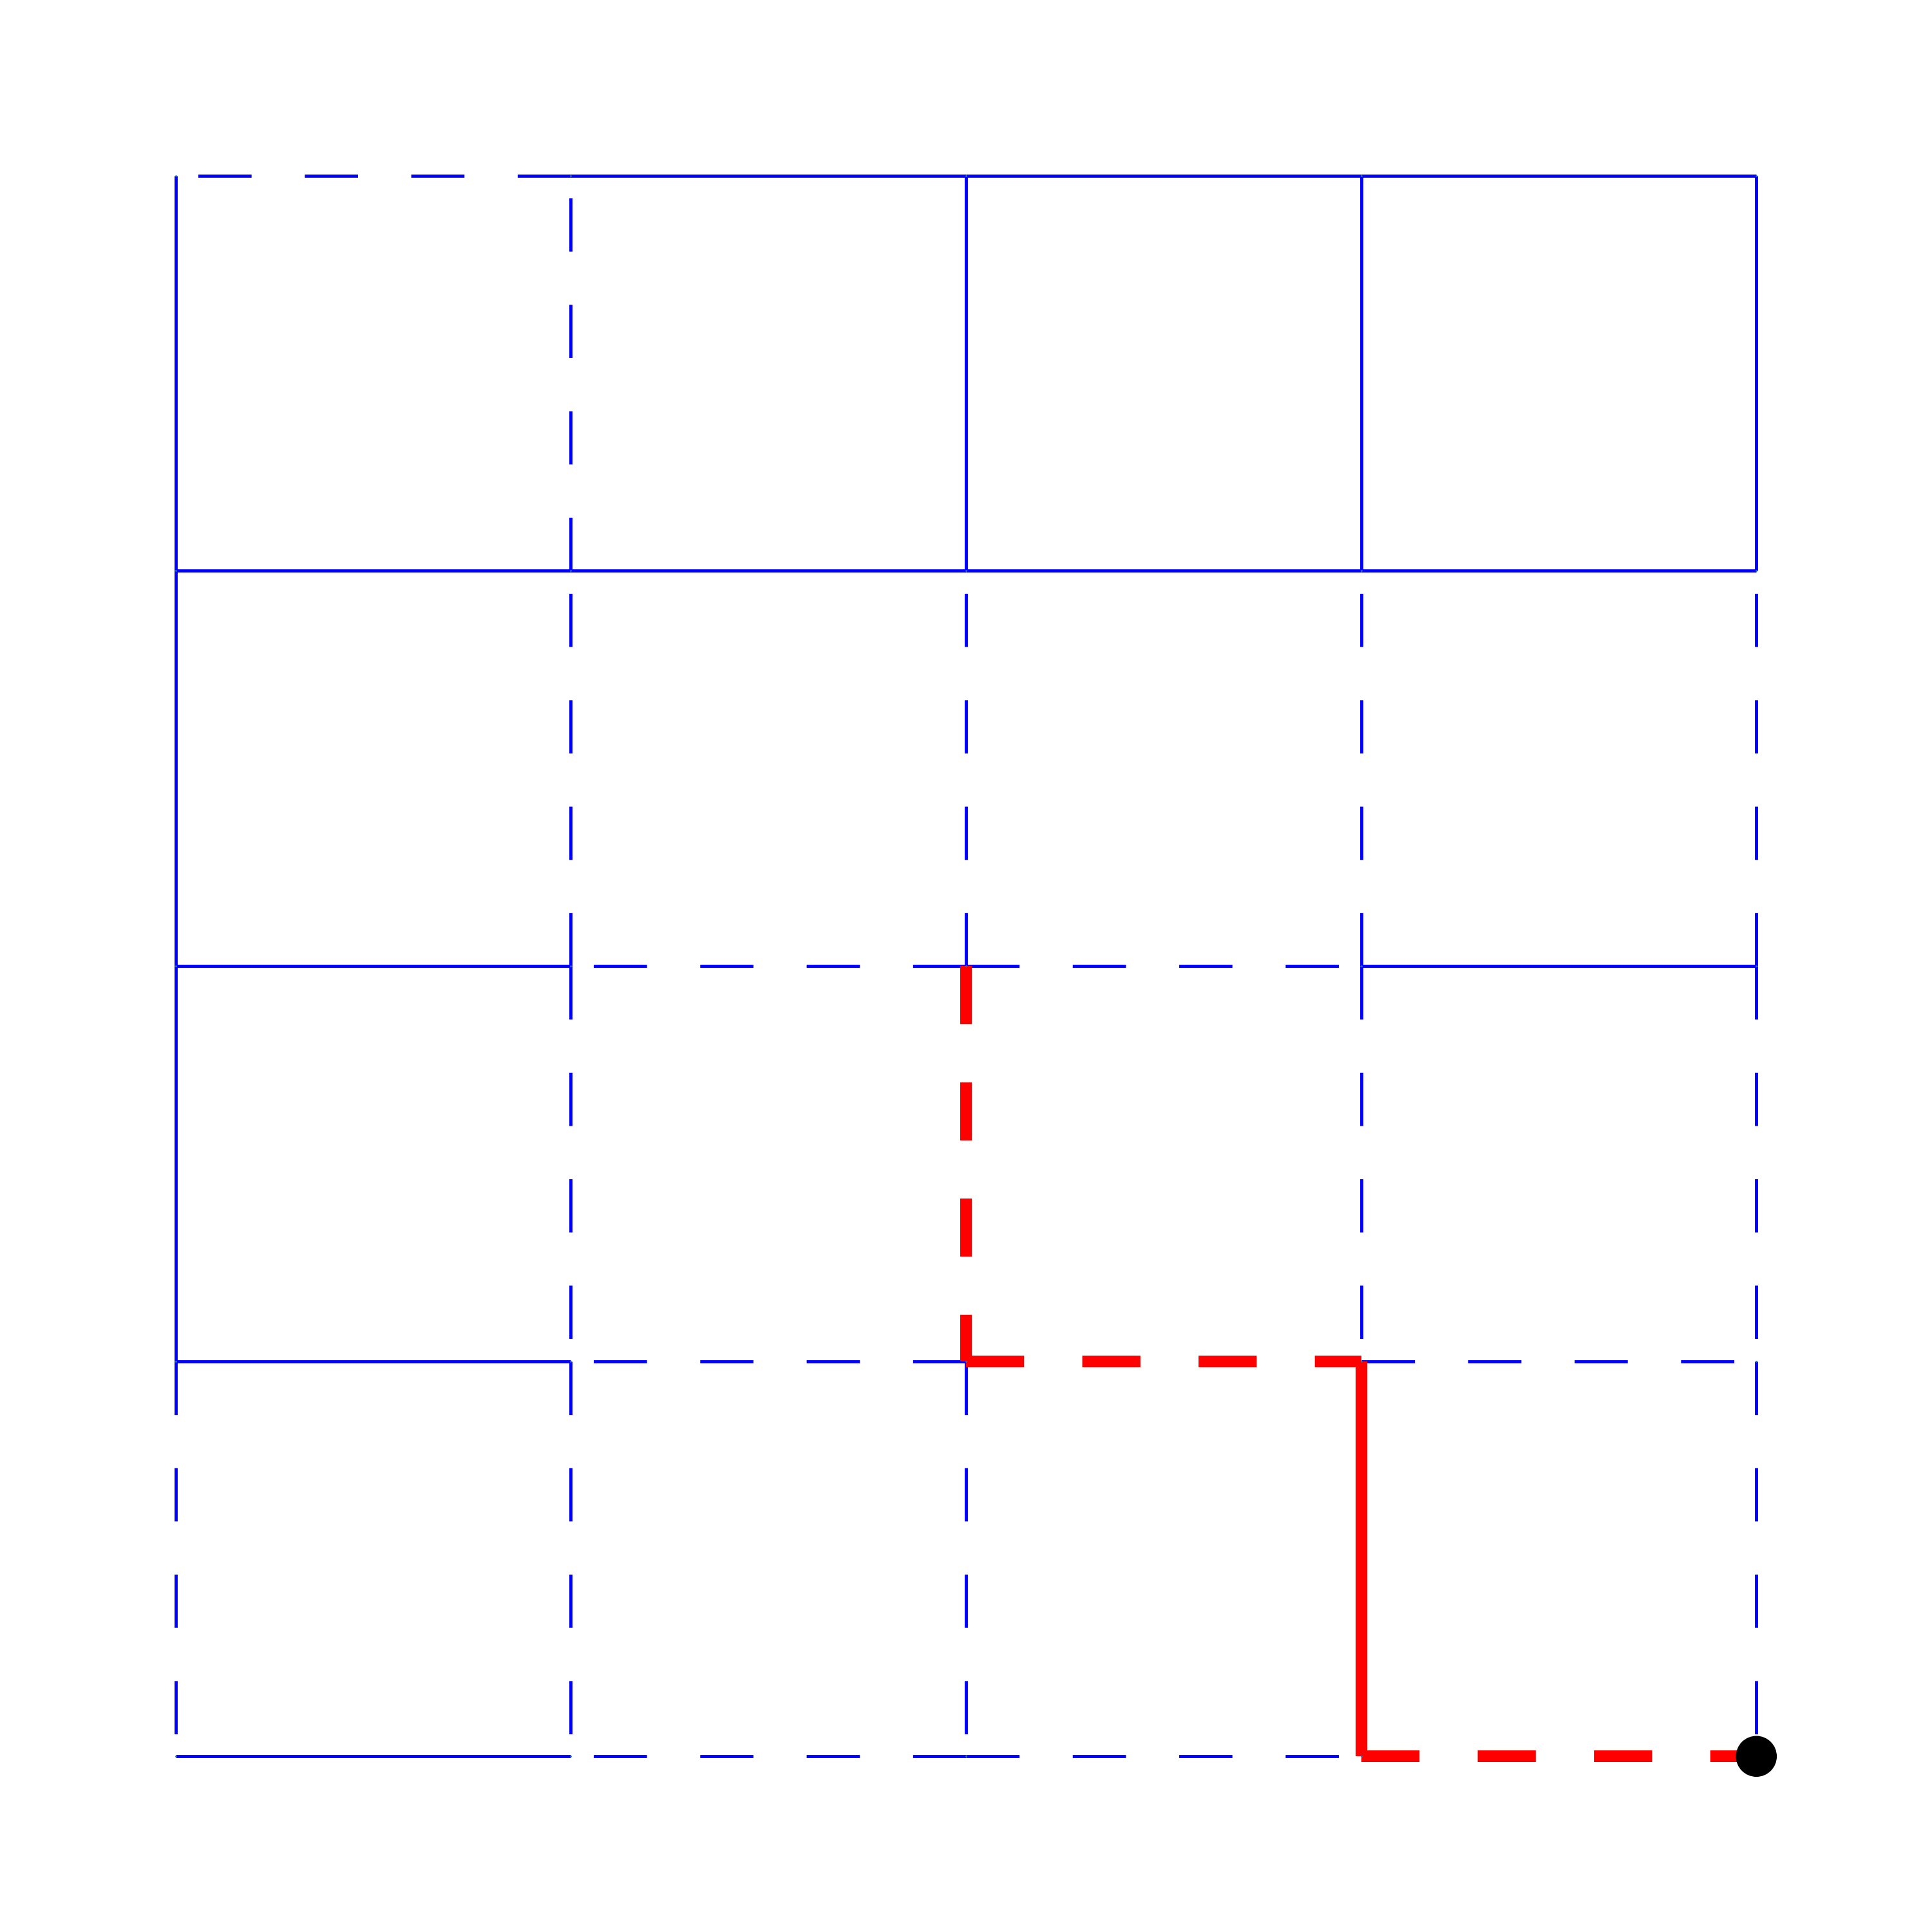
\includegraphics[width = 0.2\textwidth]{../images/game2/Ll2opit2p040.png}
            \caption{For Game 2, a realization of the payoff function for $p = 0.4$ along with the corresponding $1$-stage and 2-stage games starting from 0.}
        \end{figure}

        In essence, at each stage, player 1 moves the token up or down, then, knowing player 1's action, player 2 moves the token left or right, and both players receive the payoff associated with the edges traversed by the token.

        To ensure consistent payoffs on the same edge, we require that $g_{\omega}(z, i, 0) = g_{\omega}(z + (0, i), -i, 0)$ and $g_{\omega}(z, 0, j) = g_{\omega}(z + (j, 0), 0, -j)$ for all $(\omega, z, i, j) \in \Omega \times \Z^2 \times I \times J$. With this setting, the game is, like Game 1, a non-i.i.d. percolation game with very weak correlations. Of course, this game is non-oriented as well. 

        This time, for $m \in \N_+$, the path followed by the token up to stage $m$ has $2m$ edges:  $e_1, e_2, \ldots, e_{2m}$. As in the other game, we denote by $\{c(e)\}_{e \in \E^2}$ the random costs determined by the random payoff function and the strategies are defined in the same way. 

        For the $n$-stage game, the payoff function and the value function are
        \[
           \gamma_n(z, \sigma, \tau) := \frac{1}{2n}\sum_{m = 1}^{2n}c(e_m) \; \text{ and } \; v_n(z) := \max_{\sigma \in \Sigma}\min_{\tau \in T} \gamma_n(z, \sigma, \tau) = \min_{\tau \in T}\max_{\sigma \in \Sigma} \gamma_n(z, \sigma, \tau).
        \]

        The total payoff of the game is defined as well using the limit superior:
        \begin{equation}\label{payoff-game1}
            \gamma(z, \sigma, \tau) := \limsup_{n \to \infty}\frac{1}{2n}\sum_{m = 1}^{2n}c(e_m),
        \end{equation}
        and again by Martin's theorem the game has a value, equal to
        \[
            v_p(z) := \max_{\sigma \in \Sigma}\min_{\tau \in T} \gamma(z, \sigma, \tau) = \min_{\tau \in T}\max_{\sigma \in \Sigma} \gamma(z, \sigma, \tau).
        \]

        The limit value of this game, like that of Game 1, is expected to be independent of the initial state and deterministic. However, in this case, we have only been able to prove that its value depends on whether the sum of the coordinates of the initial state $z$ is even or odd. To establish this result, we follow the approach outlined by Ziliotto in \cite{Ziliotto2023}, which proves a corresponding result for Game 1, as stated in Theorem \ref{theorem-vz-independent-z-game1}.

\begin{theorem}
      Let $V_{even} := \{(x, y) \mid x+y \text{ is even}\}$ and $V_{odd} := \{(x, y) \mid x+y \text{ is odd}\}$. Then, $v_p(z) = v_p(z')$ for all $z, z' \in V_{even}$, and $v_p(z) = v_p(z')$ for all $z, z' \in V_{odd}$.  
\end{theorem}

\begin{proof}
    Let $z, z' \in V_{even}$. Assume $z'$ is on the right of $z$. 

    Let player 1 always play top and player 2 play optimally from $z$. Denote the path induced by these strategies as $\pi_{top}$. Since player 2 has only two options, left or right, $\pi_{top}$ will be a vertically oriented path from $z$ upwards.

    We claim that,
    \begin{equation}\label{inequality-v-top}
        v_p(z'') \leq v_p(z), \text{ for all $z'' \in \pi_{top} \cap V_{even}$.}
    \end{equation} 

    Indeed, let $\tau$ denote the strategy of player 2 playing optimally from $z$, and let $\sigma''$ be the strategy of player 1: play top until $z''$, then play optimally from $z''$.

    Since we are considering the limit superior criterion for aggregating the payoffs, which does not depend on any finite number of stages, all the payoffs between $z$ and $z''$ are negligible for \eqref{payoff-game1}. More formally, if $z$ and $z''$ are at distance $M$ in $\pi_{top}$, we have
    \begin{equation*}%\label{equality-gammas-z-z''}
        \gamma(z, \sigma'', \tau) = \limsup_{n \to \infty}\frac{1}{2n}\sum_{m = 1}^{2n}c(e_m) = \limsup_{n \to \infty}\frac{1}{2n}\sum_{m = M}^{2n}c(e_m) = \gamma(z'', \sigma'', \tau).
    \end{equation*}
    Because $\tau$ is optimal from $z$ and player 2 is minimizing, $v_p(z) \geq \gamma(z, \sigma'', \tau)$. Additionally, since $\sigma''$ is optimal from $z''$ and player 1 is maximizing, $\gamma(z'', \sigma'', \tau) \geq v_p(z'')$. Thus, we obtain the claimed inequality. 

    Now, assume player 1 always plays bottom and player 2 plays optimally from $z$. This time, the path $\pi_{bottom}$ will be a vertically oriented path from $z$ downwards. By following the same reasoning, we obtain that,
    \begin{equation}\label{inequality-v-bottom}
        v_p(z'') \leq v_p(z), \text{ for all $z'' \in \pi_{bottom} \cap V_{even}$.}
    \end{equation} 
    Thus, advancing through $\pi := \pi_{top} \cup \pi_{bottom}$, and more precisely through the vertices of $\pi \cap V_{even}$, in any direction only decreases the value.

    To relate $v_p(z)$ to $v_p(z')$, consider moving from $z'$ towards $z$. Start from $z'$, with player 2 always playing left and player 1 playing optimally from $z'$. Denote the path induced by these strategies as $\pi_{left}$. Since player 1 has only two options, top or bottom, there are 2 possibilities: $\pi_{left}$ either eventually crosses $\pi$ or it does not. For both cases, we claim that:
    \begin{equation} \label{inequality-zprime-zhat-z}
          v_p(z') \leq v_p(z).
    \end{equation} 
    From this, and by symmetry between $z$ and $z'$, we can conclude the desired equality: $v_p(z') = v_p(z)$ for all $z, z' \in V_{even}$.  

    Let us first analyze the case where the paths intersect. Let $\hat{z} \in \pi_{left} \cap \pi$ be the first intersection point. Note that $\hat{z} \in V_{even}$. Thus, if $\hat{z}$ is located at the top (or bottom) of $z$, by \eqref{inequality-v-top} (or \eqref{inequality-v-bottom}), we have
    \begin{equation*}
        v_p(\hat{z}) \leq v_p(z).
    \end{equation*}
    Furthermore, following the same line of reasoning as before, when proving \eqref{inequality-v-top}, but reversing players role, we obtain 
    \begin{equation*}
         v_p(\hat{z}) \geq v_p(z'). 
    \end{equation*}
    
    If $\pi_{left} \cap \pi = \emptyset$, then the only possibility is that both paths ``go in the same direction''. Therefore, $\pi_{left}$ must have either a finite number of top or bottom turns, and $\pi$ must have a finite number of right turns. Without loss of generality, assume $\pi_{left}$ contains a finite number of tops, then $v_p(z') \leq p$, and from $\pi$ we obtain that $v_p(z) \geq p$. 

    Finally, a similar approach can be applied to $z, z' \in V_{odd}$.

\end{proof}

\begin{remark} 
    This theorem establishes that $v_p$ remains the same regardless of which vertex in $V_{even}$ or $V_{odd}$ the game starts from. However, it may differ depending on whether the starting vertex belongs to $V_{even}$ or $V_{odd}$. We initially conjectured that this result could be extended to all $z \in \Z^2$, asserting that $v_p(z)$ is independent of the initial state $z \in \Z^2$. Although we initially believed we had proven this, errors were identified in the proof shortly before submission. We were unable to resolve these issues and decided to include this remark for clarity.
\end{remark}

If the value were independent on the initial state, the event $\{v_p > x\}$ would be invariant under translations (see the definition of the Percolation Games model in Section 2.1). By the ergodicity of $\Pbb_p$ (see Lemma 2.8 in \cite{DuminilCopin2018}), it would follow that $\Pbb_p(v_p > x) \in \{0, 1\}$ for all $x \in \R$, implying the existence of $c \in \R$ such that $v_p =  c$ almost surely.

Since we will continue working together during my PhD, we aim to complete the proof as soon as we begin. We believe the proof can be established by carefully considering whether it is Player 1's or Player 2's turn. A key question is whether the value when Player 1 starts is the same as when Player 2 starts.

        Similar to Game 1, we define winning structures for both players.

        \begin{definition}\label{def-right-structure-game2}
            A infinite subgraph $C = (V, E)$ of the lattice $\Z^2$ is said to be a winning structure for player 1 if, for all $z \in V$, there exists an $i \in I$ such that, for all $j \in J$, the vertices $z + (0, i)$ and $z + (j, i)$ are in $V$,  and the edges $\{z, z + (0, i)\}$, and $\{z + (0, i), z + (j, i)\}$ are in $E$. Similarly, a graph is said to be a winning structure for player 2 if, for all $z \in V$, there exists an $j \in J$ such that, for all $i \in I$,  $z + (j, 0)$ and $z + (j, i)$ are in $V$, and $\{z, z + (j, 0)\}$ and $\{z + (j, 0), z + (j, i)\}$ are in $E$.
        \end{definition}

        From the Definition \ref{def-right-structure-game2} it easily follows that:
        \begin{proposition}\label{rigtht-structure-player1-game2}
            A structure $C$ is a winning one for player 1 if and only if, from any of it vertices, at least one of the following local configurations is present: 
            \begin{center}
                \begin{tikzpicture}[baseline, yshift=0.5ex, scale=0.5pt] 
                    \draw[color=black!100] (0, 0) circle (2pt);
                    \draw[color = black!100] (0, 0) -- (0, -1);
                    \draw[color = black!100] (0, -1) -- (1, -1);
                    \draw[color = black!100] (0, -1) -- (-1, -1);

                    \draw[color=black!100] (2, -1) circle (2pt);
                    \draw[color = black!100] (2, 0) -- (2, -1);
                    \draw[color = black!100] (2, 0) -- (3, 0);
                    \draw[color = black!100] (2, 0) -- (1, 0);
                \end{tikzpicture}
            \end{center}
       \noindent Similarly, for player 2 a structure $C$ is a winning one if, from any of it vertices, at least one of the following local configurations is present:
       \begin{center}
            \begin{tikzpicture}[scale=0.5pt] 
                \draw[color=black!100] (0, 0) circle (2pt);
                \draw[color = black!100] (0, 0) -- (1, 0);
                \draw[color = black!100] (1, 0) -- (1, 1);
                \draw[color = black!100] (1, 0) -- (1, -1);

                \draw[color=black!100] (-1, 0) circle (2pt);
                \draw[color = black!100] (-1, 0) -- (-2, 0);
                \draw[color = black!100] (-2, 0) -- (-2, 1);
                \draw[color = black!100] (-2, 0) -- (-2, -1);
            \end{tikzpicture}
        \end{center}
        \end{proposition}

        \begin{figure}[h]
    \centering
    \begin{tikzpicture}[scale=0.5pt]
    \def\a{-5.5}
    \def\b{10.5}

    \draw[color = black!100] (0, 2) -- (3, 2);
    \draw[color = black!100] (0, 3) -- (3, 3);

    \foreach \x in {0, ..., 3} {
        \draw[color = black!100] (\x, 2) -- (\x, 2+1);
    }

    \draw[color = black!100] (2, 1) -- (10, 1);
    \draw[color = black!100] (2, 2) -- (10, 2);

    \foreach \x in {2, ..., 10} {
        \draw[color = black!100] (\x, 1) -- (\x, 1+1);
    }

    \draw[color = black!100] (9, 2) -- (12, 2);
    \draw[color = black!100] (9, 3) -- (12, 3);

    \foreach \x in {9, ..., 12} {
        \draw[color = black!100] (\x, 2) -- (\x, 2+1);
    }

    \draw[color = black!100] (11, 3) -- (15, 3);
    \draw[color = black!100] (11, 4) -- (15, 4);

     \foreach \x in {11, ..., 15} {
        \draw[color = black!100] (\x, 3) -- (\x, 3+1);
    }

    \draw[color = black!100] (14, 4) -- (16, 4);
    \draw[color = black!100] (14, 5) -- (16, 5);

     \foreach \x in {14, ..., 16} {
        \draw[color = black!100] (\x, 4) -- (\x, 4+1);
    }

    \draw[color = black!100] (15, 5) -- (21, 5);
    \draw[color = black!100] (15, 6) -- (21, 6); 
    \foreach \x in {15, ..., 21} {
        \draw[color = black!100] (\x, 5) -- (\x, 5+1);
    }

    \draw[color = black!100] (20, 4) -- (23, 4);
    \draw[color = black!100] (20, 5) -- (23, 5); 
    \foreach \x in {20, ..., 23} {
        \draw[color = black!100] (\x, 4) -- (\x, 4+1);
    }

    \draw[color = black!100] (22, 5) -- (24, 5);
    \draw[color = black!100] (22, 6) -- (24, 6);
    \foreach \x in {22, ..., 24} {
        \draw[color = black!100] (\x, 5) -- (\x, 5+1);
    }
    \end{tikzpicture}
    \caption{Possible portion of a winning structure for player 1 in Game 2.}
    \label{fig_portion_winning_structure_player1_game2}
\end{figure}

        By the previous proposition, a possible portion of a winning structure for player 2 will resemble the one shown in Figure \ref{fig_portion_winning_structure_player1_game2}, but oriented vertically rather than horizontally. Thus, we can establish a one-to-one correspondence between each winning structure for player 1 and a corresponding winning structure for player 2 by simply reversing the orientation of the winning structures (which can be viewed as rotating it by 90 degrees).

        \begin{remark}\label{remark_structures_restricted_game2}
            Winning structures for player 1 do not necessarily have to be in the form described in Figure \ref{fig_portion_winning_structure_player1_game2}. They consist of horizontal bands, by which we mean horizontal paths of contiguous squares, but these bands can be arranged one above the other in different ways. For example, a possible portion could be:
           \begin{figure}[H]
    \centering
    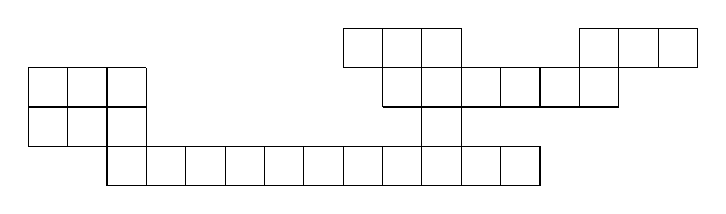
\begin{tikzpicture}[scale=0.5pt]
    \def\a{-5.5}
    \def\b{10.5}

    \draw[color = black!100] (0, 2) -- (3, 2);
    \draw[color = black!100] (0, 3) -- (3, 3);

    \foreach \x in {0, ..., 3} {
        \draw[color = black!100] (\x, 2) -- (\x, 2+1);
    }

    \draw[color = black!100] (0, 3) -- (3, 3);
    \draw[color = black!100] (0, 4) -- (3, 4);

    \foreach \x in {0, ..., 3} {
        \draw[color = black!100] (\x, 3) -- (\x, 3+1);
    }

    \draw[color = black!100] (2, 1) -- (13, 1);
    \draw[color = black!100] (2, 2) -- (13, 2);

    \foreach \x in {2, ..., 13} {
        \draw[color = black!100] (\x, 1) -- (\x, 1+1);
    }

    \draw[color = black!100] (10, 2) -- (11, 2);
    \draw[color = black!100] (10, 3) -- (11, 3);

    \foreach \x in {10, 11} {
        \draw[color = black!100] (\x, 2) -- (\x, 2+1);
    }

    \draw[color = black!100] (9, 3) -- (15, 3);
    \draw[color = black!100] (9, 4) -- (15, 4);

     \foreach \x in {9, ..., 15} {
        \draw[color = black!100] (\x, 3) -- (\x, 3+1);
    }

    \draw[color = black!100] (14, 4) -- (17, 4);
    \draw[color = black!100] (14, 5) -- (17, 5);

     \foreach \x in {14, ..., 17} {
        \draw[color = black!100] (\x, 4) -- (\x, 4+1);
    }

    \draw[color = black!100] (8, 4) -- (11, 4);
    \draw[color = black!100] (8, 5) -- (11, 5);

     \foreach \x in {8, ..., 11} {
        \draw[color = black!100] (\x, 4) -- (\x, 4+1);
    }

    % \draw[color = black!100] (15, 5) -- (21, 5);
    % \draw[color = black!100] (15, 6) -- (21, 6); 
    % \foreach \x in {15, ..., 21} {
    %     \draw[color = black!100] (\x, 5) -- (\x, 5+1);
    % }

    % \draw[color = black!100] (20, 4) -- (23, 4);
    % \draw[color = black!100] (20, 5) -- (23, 5); 
    % \foreach \x in {20, ..., 23} {
    %     \draw[color = black!100] (\x, 4) -- (\x, 4+1);
    % }

    % \draw[color = black!100] (22, 5) -- (24, 5);
    % \draw[color = black!100] (22, 6) -- (24, 6);
    % \foreach \x in {22, ..., 24} {
    %     \draw[color = black!100] (\x, 5) -- (\x, 5+1);
    % }
    \end{tikzpicture}
\end{figure}
        \end{remark}

        Let us define 41-horizontal structures as winning structures for player 1, filled with 1s. Denote by $H_{41}$ the event of its existence and define its critical probability as
        \[
            q_1 := \inf \{p \in [0, 1] : \Pbb_p(H_{41}) = 1\}.
        \]
        Similarly, we define 40-vertical structures as winning structures for player 2, filled with 0s, with $V_{40}$ denoting the event of its existence and $q_0$ representing its critical probability.

       The subscripts should be understood to indicate structures that contain 4 ones and 4 zeros, respectively. In the next subsection, a more general definition will be provided, which will clarify the reasoning behind these designations.
       
        \begin{theorem}\label{theorem-v0-q0-v1-q1}
            For all $p > q_1$, $v_p = 1$ and for all $p < q_0$, $v_p = 0$.
        \end{theorem}
        \begin{proof}
            If $p > q_1$, a $41$-horizontal (or if $p < q_0$, a $40$-vertical) structure appears. Player 1 (or player 2) can reach such a structure in a finite number of stages. Since this structure is a winning one for player 1 (or player 2), it guarantees a value of $1$ (or 0). Therefore, $v_p =  0$ for $p < q_0$ and $v_p =  1$ for $p > q_1$. 

        \end{proof}

       By the previously mentioned one-to-one correspondence between structures, we have:
       \begin{proposition}\label{proposition-relation-q0-q1}
            $q_0 = 1 - q_1$.
       \end{proposition}

       We are interested in the appearance of these structures in non-trivial cases. To this end, we need to prove the following:
       \begin{theorem}\label{theorem-q0}
            $0 < q_1 < 1$.
       \end{theorem}

       Before proving this theorem, let us define the following structures:
       \begin{definition}\label{definition_structures_restricted_game2}
            A winning structure for player 1 is said to be $41^*$-horizontal if it is a 41-horizontal structure and when viewed from left to right: 
            \begin{itemize}
                \item[--] Each square can only have neighbors to its right, above or bellow.
                \item[--] If a square has a neighbor above or below, the next square must be to the right.
            \end{itemize}
            % Similarly, a winning structure for player 2 is considered $40^*$-vertical if it is a 40-vertical structure and when viewed from top to bottom: each square can only have neighbors below, to its left, or to its right; if a square has a neighbor to the left or right, the next square must always be bellow.
        \end{definition}
        \noindent Let us further define the event of its existence as $H_{41}^*$, and $q^*_1$ as its critical probability.

        What we aim to achieve with this definition is to consider only 41-horizontal structures that are oriented in such a way that they can be traversed without retracing steps or encountering squares without lateral neighbors. In other words, we are defining structures that resemble the one shown in Figure \ref{fig_portion_winning_structure_player1_game2}, but not the one depicted in Remark \ref{remark_structures_restricted_game2}.

       We have the following relation:
       \[
            H_{41}^* \subset H_{41}.
       \]
       Therefore, $q_1 \leq q_1^*$, and hence, to prove the second inequality of Theorem \ref{theorem-q0}, it is sufficient to show $q_1^* < 1$. Moreover, by the relation in Proposition \ref{proposition-relation-q0-q1} and since $p \mapsto v_p$ is non-decreasing (see Remark \ref{remark_v_p_non_decreasing}), we have
       \begin{eqnarray*}
            q_1 < 1 \text{ and } q_0 \leq q_1 & \implies & q_0 < 1, \\
            q_0 < 1 \text{ and } q_1 = 1 - q_0  & \implies & q_1 > 0.  
       \end{eqnarray*}
        Finally, for proving Theorem \ref{theorem-q0} is enough to prove $q_1^* < 1$. 

        \begin{proof}
            For this, we use again a \emph{Peierls-type argument}. 

            % The Peierls argument, originally developed by physicist Rudolf Peierls for the 2D Ising model, has proved to be a powerful technique in statistical mechanics and percolation theory for establishing bounds on critical parameters and proving the existence of phase transitions, particularly in low-dimensional systems. 

            We refer to a face-square simply as a square and a 1-square denotes a square where all four surrounding edges are equal to 1. The length of a structure is defined as the number of squares it contains, and the distance between two squares is measured as the distance between their centers. 

            Let each square be associated with its center, and define a center as open if and only if the corresponding square is a 1-square. As in game 1, the problem of finding a path in this percolation setting --where paths consists of squares with edges that can be either open or closed-- translates into finding a path in a 1-independent site percolation model. In the following, we will use the terms squares and sites in the dual lattice interchangeably.

            Consider the dual lattice $(\tilde{\mathbb{Z}}^2, \tilde{\mathbb{E}}^2)$, constructed by assigning a vertex to each square of the original lattice and an edge between any two sites whose corresponding squares share an edge or a corner. The cost of sites in the dual lattice is determined by the state of the corresponding squares in the original lattice, as described in the previous paragraph. A dual path is defined as a sequence of vertices in the dual lattice, were each step allows for 8 possible moves (analogous to the moves of a king in a chessboard).

            \begin{figure}[!hbt]
            \centering
            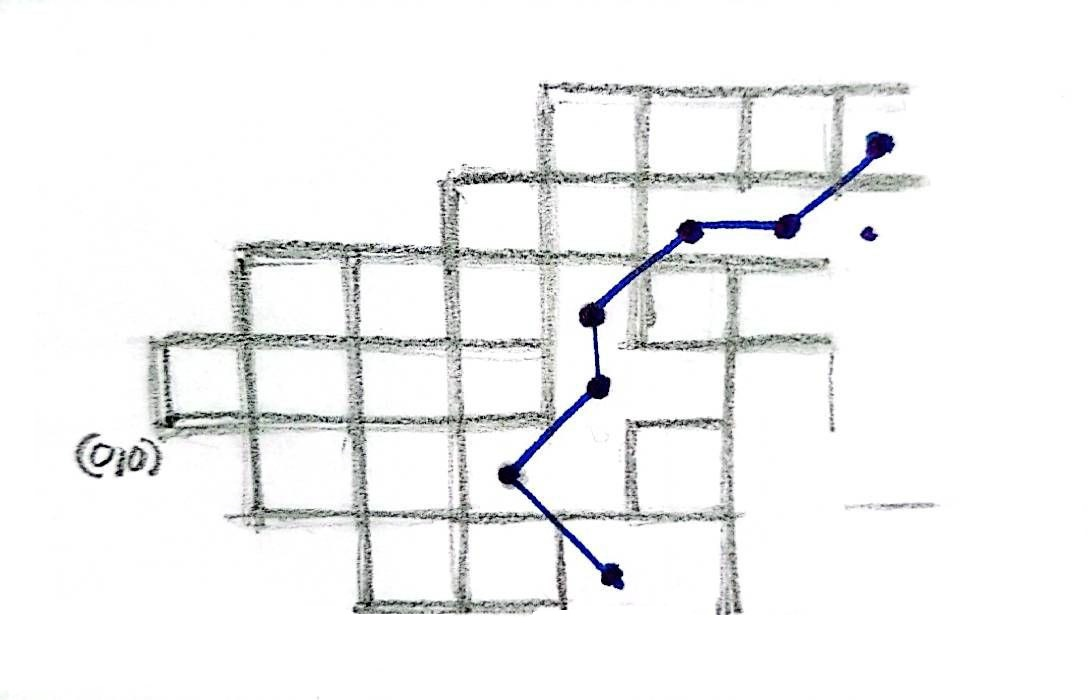
\includegraphics[width = 0.4\textwidth]{../images/game2/pierles-type-argument.jpg}
            \end{figure}

            The crucial observation is: if there is no $41^*$-horizontal structure containing the origin, there must exist an $n \in \N_+$ such that the square $[-n, n] \times [-n, n]$ is crossed vertically by a closed dual path. The previous diagram attempts to visualize this argument. The upward (or downward) dual path (represented by dark blue) is the one that `surrounds' the `tails' of the 1-square-component of the origin, preventing it from `escaping' to infinity in rightward direction.

            Another important observation is: if there is no $41^*$-horizontal, then the origin cannot be contained within one. Thus there cannot be an infinite induced path starting at 0 in the subgraph consisting of open edges.

            Using all this, the union bound, Markov inequality and the fact that a dual path from $[-n, n] \times \{n\}$ to $[-n, n] \times \{-n\}$ must have at least $2n$ edges, we obtain
                \begin{eqnarray} \notag
                   \Pbb_p(H_{41}^{*c}) & \leq & \sum_{n \geq 1} \Pbb_p\left(\substack{\text{there exist a closed dual path from}\\ [-n, n] \times \{n\} \text{ to } [-n, n] \times \{-n\}}\right) \\ \notag
                               & \leq & \sum_{n \geq 1} \E_p\left(\substack{\text{number of closed dual paths from} \\ [-n, n] \times \{n\} \text{ to } [-n, n] \times \{-n\}}\right) \\ \label{probdualpathsareclosed}
                               & \leq & \sum_{n \geq 1} n^2 \sum_{l \geq 2n} \kappa(l) \Pbb_p\left(\substack{\text{all sites of a given dual path} \\ \text{of length $l$ are closed}}\right),
                \end{eqnarray}   
            where $n^2$ accounts for the number of possible starting sites of the dual path and $\kappa(l) := \#\{\text{dual paths of length } l \text{ starting from a given square}\}$.

            Next, we provide an upper bound expression for $\kappa(l)$, which yields the bound $4^{l+2}$. 

            First, observe that traveling in one of the diagonal directions can always substitute a `corner' configuration (i.e., right then up, or left then up, or vice versa). Additionally, going in the left diagonal direction once and then right, or in the right diagonal direction once and then left (and vice versa in both situations), can be substituted by going up.

            Since we are counting the upward dual paths starting from a given fixed site (or square), we have $\kappa(1) = 1$. For $l = 2$, there are 5 possibilities: after fixing the first square, the second square can be placed in 5 different positions relative to it: above, to the right, to the left, right-up, or left-up. The last two account for the two diagonals going in the upward direction. Following this reasoning and recalling the previous observation, we obtain the following:
            \[
                \kappa(l) \leq 15\kappa(l - 2),\; \text{  for $l \geq 3$, }
            \] 
            where the term accounts for placing the second square above (which then has only 3 possibilities for the third), to the right (which has only 2 possibilities), to the left (which has also 2 possibilities), or to the left-up or right-up (which has 4 possibilities).

            Now, let $\tilde{\alpha}$ be the given oriented dual path of length $l$. For any square in $\tilde{\alpha}$, there are at most two squares in the path that share an edge with it. According to the previous analysis used to reduce the types of dual paths we are looking for, this can only happen in horizontal or vertical sequences of sites. Hence, there exists a sub-path $\tilde{\beta}$ consisting of at least $l/2$ squares from $\tilde{\alpha}$ such that any two squares $x, y \in \tilde{\beta}$ are at a distance greater than 1. Between these paths, $\tilde{\alpha}$ and $\tilde{\beta}$, the following relation holds:
            $$
                \Pbb_p(\text{every square in } \tilde{\alpha} \text{ is not a 1-square}) \leq \Pbb_p(\text{every square in } \tilde{\beta} \text{ is not a 1-square}).
            $$ 
            Moreover, since the costs of the squares of $\tilde{\beta}$ are independent, we get
            \[
                \Pbb_p(\text{every square in } \tilde{\alpha} \text{ is not a 1-square}) \leq (1 - p^4)^{|\tilde{\beta}|} \leq (1 - p^4)^{l/2}. 
            \]

            Consequently, 
            \[
                \Pbb_p(H_{41}^{*c}) \leq \sum_{n \geq 1} n^2\sum_{l \geq 2n}  4^{l+2} (1 - p^4)^{l/2} \to 0 \text{ as } n \to \infty \text{ for } p \text{ sufficiently large}.
            \]

            Hence, for $p$ in the interval $((15/16)^{1/4}, 1)$, we have
            \[
                \Pbb_p(H_{41}^{*c}) < 1, \text{ and thus } \Pbb_p(H_{41}^*) > 0.
            \] 
            Since the event $H_{41}^*$ is translation invariant, we can conclude that $q _1^* \leq \frac{\sqrt[4]{15}}{2}\approx 0.98 < 1$.

        \end{proof}

        We finally claim the following conjecture. 
        \begin{conjecture}\label{conjecture-v0-q0}
           $v_p = 1$ if and only if $p \geq q_1$, and $v_p = 0$ if and only if $p \leq q_0$.
        \end{conjecture}
        The same comments as for Conjecture \ref{conjecture-v0-p0} apply here. However, it is worth noting that the winning structures in this game appear simpler than the winning structures for player 1 in Game 1. Consequently, we expect that the proofs may be simpler.

        % For this game, we could think that these are the only two key points or phase transitions for the game's value. 
        In the next section we will see, with the help of computational methods, how the value function of this game has more than 2 phase transitions.

    \subsection{Computational findings}
        % For both games, we also consider to approximate the critical probability tresholds of all the relevant structures by simulating the games. The algorithm that we use for estimate the expected value fot the limit value of the game is quite slow but one possible future research direction could be to develop it optimally.

        We simulated both games to estimate the expected value of $v_n$ as a function of $p$ for each game, with $n$ as large as our computers could handle. This section aims to briefly describe the computational methods employed for these simulations and discuss the results obtained. We begin by presenting the results for Game 2, as they provide significant new insights into the behavior of its limit value. For Game 1, although we know more about it, it was still valuable to approximate the value of $p_0$ and observe how the value of $p$ behaves between $p_0$ and $p_1$. 
        
        All the computer programs used are being prepared for upload to a public repository. We decided not to include them in the report due to their length. In the meantime, you can contact me\footnote{At the email address melgonzalez073@gmail.com}. We will be happy to share them with you and discuss them, if needed.

        To estimate the expected value of $v_n$ as a function of $p$, we followed the approach: We fixed a finite two-dimensional lattice and a sequence of 200 equally spaced $p$ values within the interval $(0, 1)$. For each $p$, we ran 30 simulations with independent and identically distributed realizations of the costs on the edges. For each fixed realization, we computed the value of the largest finite stage game starting at the center of the finite lattice and constrained within its boundaries, using a recursive method.
        
        \subsubsection*{Game 2}
        Let $\mathcal{L} := [-N..N] \times [-N..N]$ be the finite square portion of $\Z^2$ centered at $0$, and let $(C_{i, j, a, b})$, where $(i, j, a, b) \in \mathcal{L} \times \{ (1, 0), (-1, 0), (0, 1), (0, -1)\}$, denote the payoff of the edge between $(i, j)$ and $(i + a, j + b)$. 

        For a fixed $p$ in $(0, 1)$, we generate the costs by independently assigning a cost of 1 to each edge of $\mathcal{L}$ with probability $p$. For each fixed realization of the costs, determining the optimal strategy for the players in the $n$-stage game can be approached recursively, as well as the computation of the value. 

        \begin{figure}[!hbt]
        \centering
            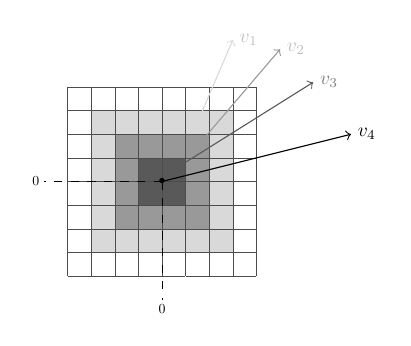
\begin{tikzpicture}[scale=0.6pt]                    
                \fill[thick,fill=gray!30] (-1.5, -1.5) -- (1.5, -1.5) -- (1.5, 1.5) -- (-1.5, 1.5);
                \fill[thick,fill=gray!80] (-1, -1) -- (1, -1) -- (1, 1) -- (-1, 1);
                \fill[thick,fill=gray!130] (-0.5, -0.5) -- (0.5, -0.5) -- (0.5, 0.5) -- (-0.5, 0.5);
                
                % Define the color and line thickness for easy reference
                \pgfkeys{/
                  my/.style={
                    line width=0.5pt,
                  }
                }

                \foreach \x in {-2., -1.5, -1., -0.5, 0, 0.5, 1, 1.5, 2.} {
                    \foreach \y in {-2., -1.5, -1, -0.5, 0, 0.5, 1., 1.5, 2.} {
                        % Determine color based on the x coordinate
                        \pgfmathsetmacro{\color}{(\x == 2 ? "white" : "black!70")}
                            \draw[ultra thin, color=\color] (\x, \y) -- (\x + 0.5, \y);
                        \pgfmathsetmacro{\color}{(\x == -2 ? "white" : "black!70")}
                            \draw[ultra thin, color=\color] (\x, \y) -- (\x - 0.5, \y);                         
                        \pgfmathsetmacro{\color}{(\y == 2 ? "white" : "black!70")}
                            \draw[ultra thin, color=\color] (\x, \y) -- (\x , \y + 0.5);                            
                        \pgfmathsetmacro{\color}{(\y == -2 ? "white" : "black!70")}
                            \draw[ultra thin, color=\color] (\x, \y) -- (\x, \y - 0.5);

                    }
                }

                \coordinate (a) at (0., 0);
                \coordinate (v) at (0., -2.5);
                \coordinate (h) at (-2.5, 0.);
                \draw[dashed, ultra thin, color=black](a)node{} -- (v)node[below, color=black, scale=0.5pt]{0};
                \draw[dashed, ultra thin, color=black](a)node{} -- (h)node[left, color=black, scale=0.5pt]{0};

                \coordinate (b) at (0. , 0.);
                \coordinate (b') at (4, 1.);
                \draw[->](b)node[scale=0.5pt]{$\bullet$}--(b')node[right, scale=0.7pt]{$v_4$};

                \coordinate (b) at (0.25 , 0.25);
                \coordinate (b') at (3.2, 2.1);
                \draw[->, color=gray!130](b)node{} -- (b')node[right, color=gray!100, scale=0.7pt]{$v_3$};

                \coordinate (b) at (0.75, 0.75);
                \coordinate (b') at (2.5, 2.8);
                \draw[->, color=gray!80](b)node{} -- (b')node[right, color=gray!50, scale=0.7pt]{$v_2$};

                \coordinate (b) at (0.75, 1.25);
                \coordinate (b') at (1.5, 3);
                \draw[->, color=gray!30](b)node{} -- (b')node[right, color=gray!50, scale=0.7pt]{$v_1$};
            \end{tikzpicture}
            \caption{Representation of the recursion for $N = 4$. From a specific vertex, the largest stage game that can be played from it depends on how deep it is towards the center. This is represented using a scale of gray colors. The value of the vertices in the strongly colored areas depends on the lighter areas that surround them.}
        \end{figure} 

        Suppose we are at stage $n$ and player 1 has already played, moving the token to $(i', j')$. Player 2 is now deciding what to play. Player 2's choice depends on the value of the $(n-1)$-stage games starting at positions $(i'+ 1, j')$ and $(i'-1, j')$. If player 2 moves right, the cost will be
        \begin{equation}\label{player2-right}
            C_{i, j', 1, 0} + v_{n-1}(i'+1, j'),
        \end{equation}
        whereas if player 2 moves left, the cost will be 
        \begin{equation}\label{player2-left}
            C_{i, j', -1, 0} + v_{n-1}(i'-1, j').
        \end{equation}
        Hence, he will choose the minimum between these 2 expressions. 

        Now, consider being at position $(i, j)$ at stage $n$ in player 1's turn. If player 1 moves up, he will receive the cost of the edge from $(i, j)$ to $(i, j + 1)$ plus the minimum between \eqref{player2-right} and \eqref{player2-left} with $(i', j') = (i, j+1)$. A similar analysis applies if player 1 moves down. Therefore, the value of the $n$-stage game starting at $(i, j)$ can be computed using the recursion: 
        \begin{align*}   
            v_n(i, j) = & \max (C_{i, j, 0, 1} + \min (C_{i, j+1, 1, 0} + v_{n-1}(i+1, j+1), C_{i, j+1, -1, 0} + v_{n-1}(i-1, j+1)), \\
                        & C_{i, j, 0, -1} + \min (C_{i, j-1, 1, 0} + v_{n-1}(i+1, j-1), C_{i, j-1, -1, 0} + v_{n-1}(i-1, j-1))).
        \end{align*}

        The initialization of this recursion should be done on the boundaries since as you move deeper into the lattice, you can play more stages. When starting at $(i, j)$, it is only meaningful to consider games up to $N - \max(\lvert i\rvert , \lvert j\rvert )$ stages. If you attempt to play more than this, the token may reach a point where not all 4 moves are available.

        \begin{figure}[!hbt]
            \centering
            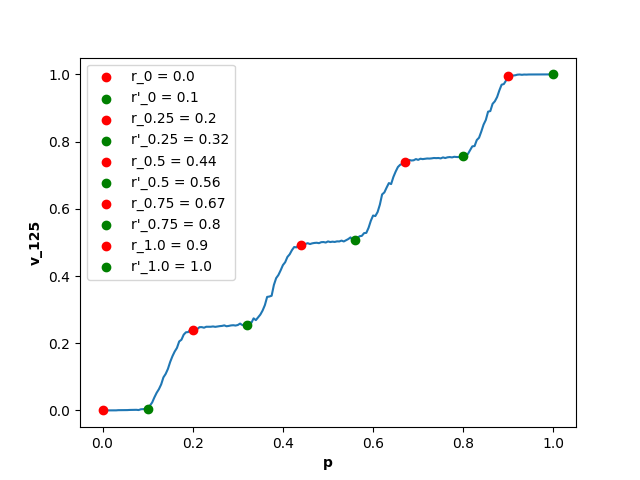
\includegraphics[width = 0.31\textwidth]{../images/game2/pN125MAXITER30.png}        
            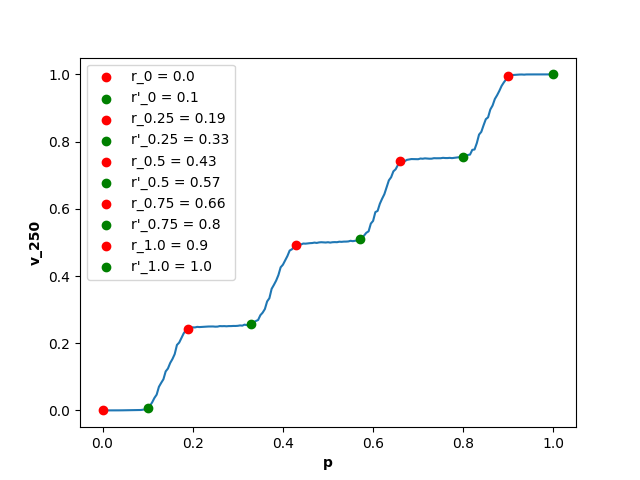
\includegraphics[width = 0.31\textwidth]{../images/game2/pN250MAXITER30.png}        
            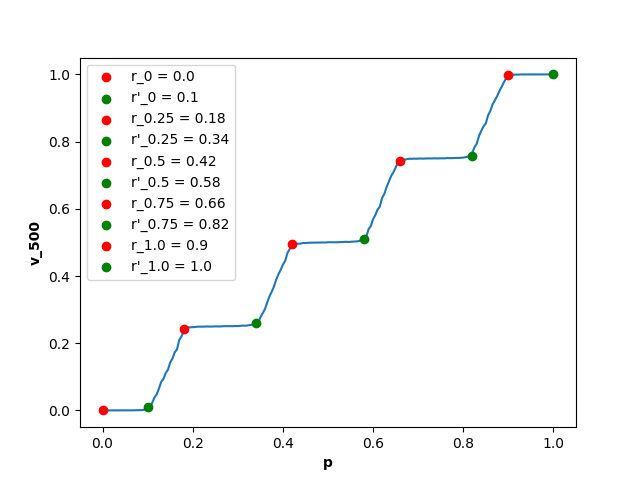
\includegraphics[width = 0.31\textwidth]{../images/game2/pN500MAXITER30.png}
            \caption{For Game 2, $v_{n}$ is plotted as a function of $p$ for $n = 125, 250$ and $500$. Red points represent the approximate lower values of $p$ at which the function value is within a distance less than a threshold, fixed  by us at 0.01, from 0, 0.25, 0.5, 0.75 and 1, respectively, while green points indicate the corresponding upper values of $p$.}
           \label{figurepNgame2}
        \end{figure} 

        From the simulations, we obtain the graphs in Figure \ref{figurepNgame2}.

        They are quite striking, showing that the value function almost stabilizes at 0, 0.25, 0.5, 0.75, and 1 for intervals determined by probability thresholds, indicated by the red and green points. This suggests the occurrence of eight phase transitions.

        Let define $r_{x}$ and $r'_{x}$ for $x \in \{0, 0.25, 0.5, 0.75, 1\}$ as the probability thresholds between which $v_p$ is almost surely equal to $x$, i.e.,
        \begin{equation*}
            r_x := \inf\{p \in [0, 1] \colon \Pbb_p(v_p =  x) = 1\}, \; \text{and} \; r_x' := \inf\{p \in [0, 1] \colon \Pbb_p(v_p > x) = 1\}.
        \end{equation*}
       By the one-to-one correspondence between the players' winning structures, and therefore between their strategies, we should have $r_x = 1 - r_{1-x}'$ for all $x \in \{0, 0.25, 0.5, 0.75, 1\}$. Thus, from now on, everything discussed will be with respect to the $r_x$'s.
        
        It is expected that these thresholds correspond to the critical probabilities for some specific structures. In particular, we should have the following.

        \begin{conjecture}\label{conjecture_q1_r1}
            $r_1 = q_1$.
        \end{conjecture}

        Indeed, since the function $p \mapsto v_p$ is non-decreasing, we have, in particular,
        $$
            q_1 = \sup \{p \in [0, 1] \colon \Pbb_p(H_{41}) < 1\}.
        $$ 
        On the other hand, from Conjecture \ref{conjecture-v0-q0} we would have
        $$
            q_1 = \inf \{p \in [0, 1] \colon \Pbb_p(v_p = 1) = 1\}.
        $$
        
        Let us define $km$-horizontal structures for $k \in \{0, 1, 2, 3, 4\}$ and $m \in \{0, 1\}$ as those satisfying the conditions of Proposition \ref{rigtht-structure-player1-game2}, where all the squares composing them have $k$ or more $m$'s. We denote their event of existence as $H_{k1}$.  In particular, a square with 2 ones in a $21$-structure can take one of the following forms: 
        \begin{center}
            \begin{tikzpicture}[baseline, yshift=-0.7ex] 
                % \node at (0,0) [square, draw, scale=1.8pt] (square) {};
                \draw[dashed, thin, color = blue] (0.5, 0.5) -- (1, 0.5);
                \draw[thin, color = blue] (1, 0.5) -- (1, 0);
                \draw[dashed, thin, color = blue] (1, 0) -- (0.5, 0);
                \draw[thin, color = blue] (0.5, 0) -- (0.5, 0.5);
            \end{tikzpicture}
            \, 
            \begin{tikzpicture}[baseline, yshift=-0.7ex] 
                % \node at (0,0) [square, draw, scale=1.8pt] (square) {};
                \draw[thin, color = blue] (0.5, 0.5) -- (1, 0.5);
                \draw[dashed,thin, color = blue] (1, 0.5) -- (1, 0);
                \draw[dashed, thin, color = blue] (1, 0) -- (0.5, 0);
                \draw[thin, color = blue] (0.5, 0) -- (0.5, 0.5);
            \end{tikzpicture}
            \,
            \begin{tikzpicture}[baseline, yshift=-0.7ex] 
                % \node at (0,0) [square, draw, scale=1.8pt] (square) {};
                \draw[dashed, thin, color = blue] (0.5, 0.5) -- (1, 0.5);
                \draw[dashed, thin, color = blue] (1, 0.5) -- (1, 0);
                \draw[thin, color = blue] (1, 0) -- (0.5, 0);
                \draw[thin, color = blue] (0.5, 0) -- (0.5, 0.5);
            \end{tikzpicture}  
            \,
            \begin{tikzpicture}[baseline, yshift=-0.7ex] 
                % \node at (0,0) [square, draw, scale=1.8pt] (square) {};
                \draw[dashed, thin, color = blue] (0.5, 0.5) -- (1, 0.5);
                \draw[thin, color = blue] (1, 0.5) -- (1, 0);
                \draw[thin, color = blue] (1, 0) -- (0.5, 0);
                \draw[dashed, thin, color = blue] (0.5, 0) -- (0.5, 0.5);
            \end{tikzpicture}
            \,
            \begin{tikzpicture}[baseline, yshift=-0.7ex] 
                % \node at (0,0) [square, draw, scale=1.8pt] (square) {};
                \draw[thin, color = blue] (0.5, 0.5) -- (1, 0.5);
                \draw[thin, color = blue] (1, 0.5) -- (1, 0);
                \draw[dashed, thin, color = blue] (1, 0) -- (0.5, 0);
                \draw[dashed, thin, color = blue] (0.5, 0) -- (0.5, 0.5);
            \end{tikzpicture}
            \,
            \begin{tikzpicture}[baseline, yshift=-0.7ex] 
                % \node at (0,0) [square, draw, scale=1.8pt] (square) {};
                \draw[thin, color = blue] (0.5, 0.5) -- (1, 0.5);
                \draw[dashed, thin, color = blue] (1, 0.5) -- (1, 0);
                \draw[thin, color = blue] (1, 0) -- (0.5, 0);
                \draw[dashed, thin, color = blue] (0.5, 0) -- (0.5, 0.5);
            \end{tikzpicture} 
        \end{center}

        \begin{conjecture}\label{conjecture-r-q}
                \begin{align}
                    r_{0.25} & = \inf\{p \in [0, 1] \colon \Pbb_p(H_{11}) = 1\} \\
                    r_{0.5}  & = \inf\{p \in [0, 1] \colon \Pbb_p(H_{21}) = 1\} \\
                    r_{0.75} & = \inf\{p \in [0, 1] \colon \Pbb_p(H_{31}) = 1\}
                \end{align}  
        \end{conjecture}
        
        This conjecture states that $v_p \geq x$  if and only if a  $k1$-structure with $k \geq 4x$ appears; that is, if a winning structure for player 1 with squares having \( 4x \) or more 1s emerges. Specifically, $v_p \geq 0.25$ if and only if the number of 1s in each square of the winning structure is 1 or more. 

        Returning to Figure \ref{figurepNgame2}, one possible interpretation of the graphs based on this conjecture is as follows: From $r_0$ to $r_0'$, player 1 cannot achieve more than zero, as for $p < r_0'$, player 2 guarantees a winning structure filled with 0s. After $r_0'$ and up to $r_{0.25}$, player 1 will try to find structures with as many 1s as possible, which explains the increase up to $r_{0.25}$. Beyond $r_{0.25}$ and up to $r_{0.25}'$, the value no longer increases because, once again, for $p < r_{0.25}'$, player 2 ensures a winning structure with squares having 3 or more 0s (or having 1 or fewer 1s). This pattern continues through the analysis up to $r_1'$. Hence, player 1 consistently strives to obtain more 1s, but at certain points, player 2 halts his progress, forcing player 1 to settle for fixed values.

        In an effort to test these conjectures, we computationally investigated the critical probability of the appearance of winning structures containing $k$ or more 1s. Instead of studying the percolation probability for the events $H_{k1}$, we considered the events $H_{k1}^*$, as defined in the previous section (see Definition \ref{definition_structures_restricted_game2} and the subsequent analysis). We chose this approach not only because it simplified the computational analysis but also because we believe these structures are either the relevant ones or very close to them. In the following, we refer to a $k$-square as a square with $k$ or more 1s.

        In this phase of the analysis, the game is no longer considered. Instead, we focus on the percolation model on the square lattice $\Z^2$ and aim to identify a connected graph of $k$-squares that meets the conditions of Definition \ref{definition_structures_restricted_game2} and spans the lattice from the left side to the right side, thereby estimating the right-hand sides of the equations in Conjectures \ref{conjecture-r-q} and \ref{conjecture_q1_r1}. From now on, we refer to connected graphs as clusters.

        We utilized a modified version of the Newman-Ziff algorithm, as proposed by Newman and Ziff \cite{NewmanZiff2001}, which allows us to measure observable quantities (e.g., average cluster size, largest cluster size, or cluster spanning) in a percolation system across all values of site or bond open probability, from zero to one. The algorithm, described here in terms of bond percolation, is based on a simple yet powerful idea: creating a set of percolation configurations by opening bonds one by one, starting from a lattice with all bonds initially closed. Additionally, the clusters on the lattice change minimally when a single bond is opened, enabling the computation of new clusters from the old ones with relatively little computational effort. To track the cluster configuration of the lattice, the algorithm employs a method called union-find, which efficiently performs the following operations: when a bond is opened, it finds which clusters the sites at either end belong to; if the sites belong to different clusters, those clusters are unified into a single cluster. If the sites are already in the same cluster, no action is performed.

        Originally developed to handle (non-oriented) site or bond percolation, the algorithm had to be adapted for our study to manage paths formed by $k$-squares that meet the conditions specified in Definition \ref{definition_structures_restricted_game2}. Briefly, we start with a lattice $\mathcal{L}$ with a fixed $N$ in which all bonds are closed. We then proceed as follows: First, we determine an order for opening the bonds by choosing a random permutation of them. With this order established, we open the bonds one by one accordingly. As bonds are opened, new clusters of single $k$-square are created, or existing clusters of $k$-squares are merged into larger ones, or nothing interesting happens, as some opened bonds may connect pairs of squares that are already in the same cluster. This process continues until all bonds on the lattice are opened. At each step, we check if a new $k$-square has been created, and if so, we verify the existence of a connected graph of squares that meets the definition. We perform this check using a combination of a union-find algorithm and a depth-first search. If such a cluster is found, we record the onset of percolation for that step, which corresponds to the mean number of open bonds. Finally, we ran 30 simulations of this procedure and averaged the results to obtain the mean onset of percolation.

        \begin{figure}[!hbt]
            \centering
            \begin{minipage}{.33\linewidth}
              \centering
                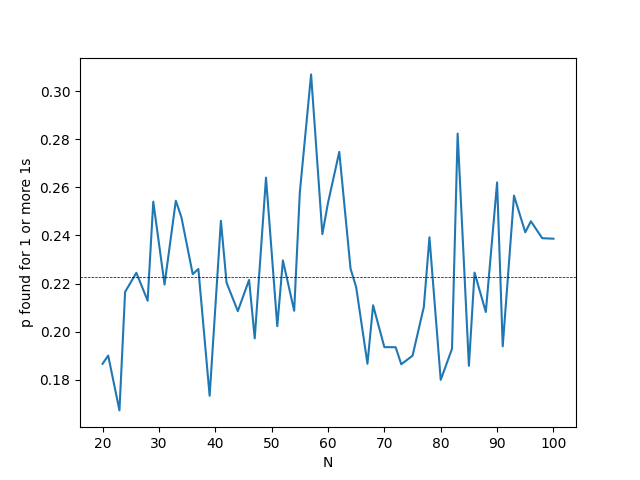
\includegraphics[width = \textwidth]{../images/game2/0001_L_vs_p_MAX_L50-5100.png}
              \caption{$k = 1$.}
              \label{figure-k1}
            \end{minipage}
            \begin{minipage}{.33\linewidth}
              \centering
                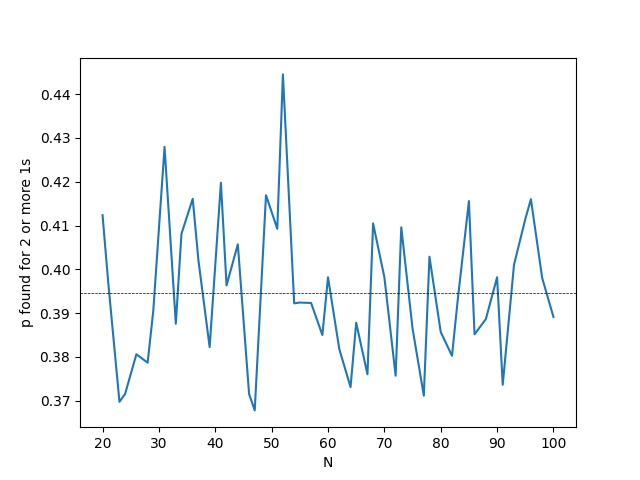
\includegraphics[width = \textwidth]{../images/game2/0011_L_vs_p_MAX_L50-5100.png}
              \caption{$k = 2$.}
              \label{figure-k2}
            \end{minipage}      
            \begin{minipage}{.33\linewidth}
              \centering
                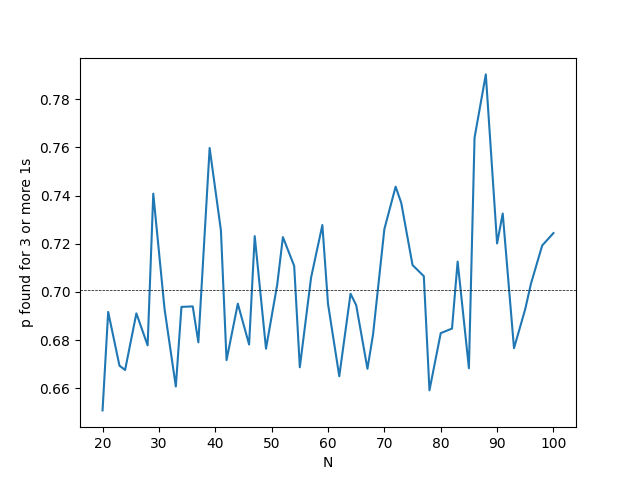
\includegraphics[width = \textwidth]{../images/game2/0111_L_vs_p_MAX_L50-5100.png}
              \caption{$k = 3$.}
              \label{figure-k3}
            \end{minipage}      
            \begin{minipage}{.33\linewidth}
              \centering
                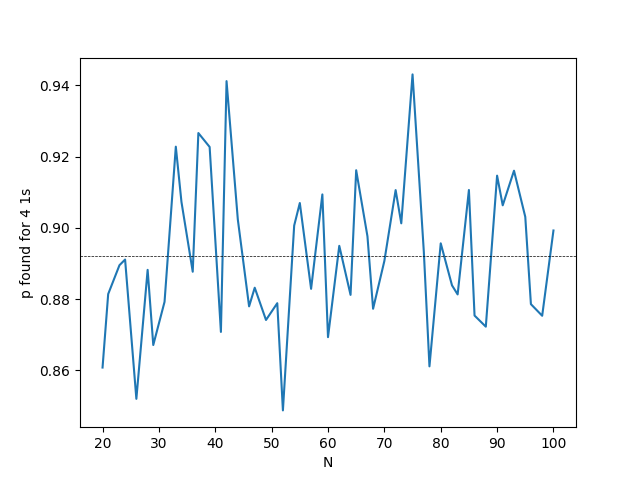
\includegraphics[width = \textwidth]{../images/game2/1111_L_vs_p_MAX_L50-5100.png}
              \caption{$k = 4$.}
              \label{figure-k4}
            \end{minipage}                     
        \end{figure} 

        The graphs in Figures \ref{figure-k1}-\ref{figure-k4} display the critical probability as a function of $N$ for four values of $k\colon 1, 2, 3$ and 4, along with their mean represented by a horizontal dashed line. The data was obtained from this algorithm for a sequence of 50 equally spaced $N$ values within the interval [20, 100].

        We observe that the range of values for each $k$ aligns quite well with the values of the red points in the graphs in Figure \ref{figurepNgame2}, which represent estimates of $r_{k/4}$ from the game simulations. We could say that, they could be slightly higher, but this does not contradict the conjecture, as the points that determine these intervals correspond to onset percolation probabilities of the events $H_{k1}^*$, which, as the analysis in the previous section shows, should be greater than those for the corresponding events $H_{k1}$.

        \subsubsection*{Game 1}
        Let $\mathcal{L} := [-N..N] \times [-N..N]$ be the finite square portion of $\Z_r^2$, centered at $0$, and $(C_{i, j, a, b})$, $(i, j, a, b) \in \mathcal{L} \times \{(1, -1), (-1, 1), (1, 1), (-1, -1)\}$ the payoff of the edge between $(i, j)$ and $(i + a, j + b)$. For a given $p$ in $(0, 1)$ and a fixed realization of the costs, the recursion for calculating the $n$-stage value of this game is
        \begin{align*}   
            v_n(i, j) =  \min (& \max (C_{i, j, 1, 1} + v_{n-1}(i+1, j+1), C_{i, j, -1, 1} + v_{n-1}(i-1, j+1)), \\
                               & \max (C_{i, j, 1, -1} + v_{n-1}(i+1, j-1), C_{i, j, -1, -1} + v_{n-1}(i-1, j-1))).
        \end{align*}

        % To generate the graph of $v_n(p)$ as a function of $p$, as for game 2, we considered 200 equally spaced $p$ values in $(0, 1)$ and for each $p$, we ran 30 simulations.

        \begin{figure}[!hbt]
            \centering
            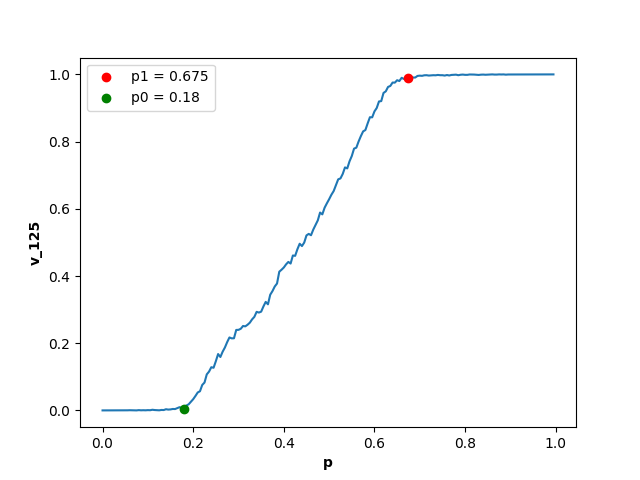
\includegraphics[width = 0.31\textwidth]{../images/game1/0pN125MAXITER30EPS0.01.png}        
            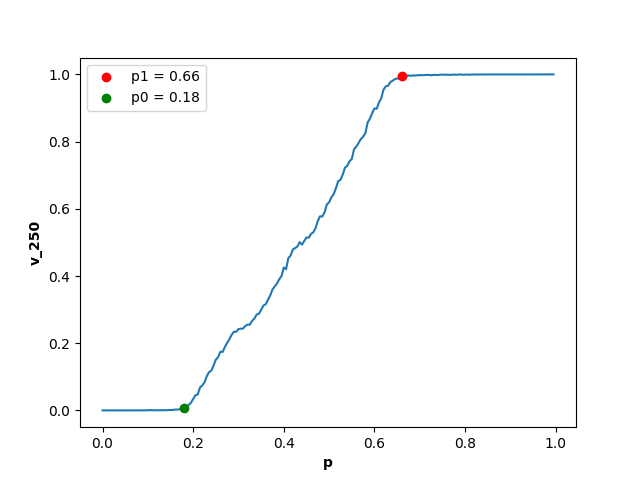
\includegraphics[width = 0.31\textwidth]{../images/game1/0pN250MAXITER30EPS0.01.png}        
            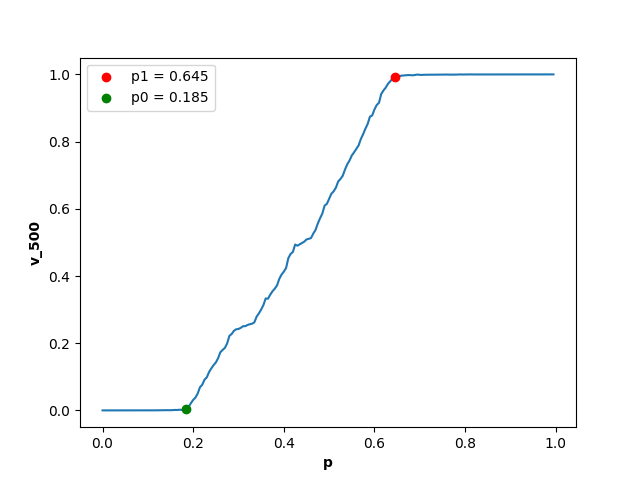
\includegraphics[width = 0.31\textwidth]{../images/game1/0pN500MAXITER30EPS0.01.png}
            \caption{For Game 1, $v_{n}$ is plotted as a function of $p$ for $n = 125, 250$ and $500$. The values at which $v_{n}$ stabilizes are 0 and 1.} 
            \label{figurepNgame1}
        \end{figure} 

        The simulations suggest that between $p_0$ and $p_1$, the value almost stabilizes again, though for a very short time, in the values $0.25$ and $0.5$. This behavior might again be related to the distribution of 0s and 1s in the squares, which could contain the winning structures for player 1. They also indicate that $0.15 < p_0 < 0.2$ and that $p_0$ converges to a value close to $0.185$. Furthermore, they suggest that the value function is continuous everywhere.

        To further investigate whether the limit value exists without the orientation assumption, the next section explores a generalization of the Percolation Games model by incorporating random noise into the game's transition function.

	 \section{Randomness in transitions}
 	In this section, we first define the generalized model and update the definition of oriented games to account for the randomness introduced in the state transition function. Then, for these new games, we prove a result equivalent to those presented in Theorem \ref{theorem_iid_and_oriented_percolation_games}.

	\subsection{Generalizing the model}
	For a percolation game $\Gamma = (I, J, \mathcal{E}, g, q)$, we consider a generalization of the model by adding a discrete-time stochastic process $\xi = (\xi_m)_{m \geq 1}$ to the game's transition function $q$, where $(\xi_m)$ is a sequence of i.i.d. discrete random variables defined on the same probability space $(\Omega, \mathcal{F}, \mathbb{P})$. In the sequel, this game is denoted by $\Gamma_{\xi} = (I, J, \mathcal{E}, g, q + \xi)$, and for a specific known common distribution $\mu$ of the $(\xi_m)$, it is denoted by $\Gamma_{\mu}$. 
	
	Given an initial state $z \in \Z^d$  and $\omega \in \Omega$, the game $\Gamma_{\xi}$ proceed in the same way as in $\Gamma$: Players are informed of $\omega$. At each stage $m \in \N_+$, player 1 chooses an action $i_m$, and then knowing player 1's action, player 2 chooses an action $j_m$. Players 1 and 2 receive respective payoffs $g_w(z_m, i_m, j_m)$ and $-g_w(z_m, i_m, j_m)$. Then, the new state updates according to the modified transition function 
	\[
		z_{m+1} := z_m + q(i_m, j_m) + \xi_{m}.
	\]
	
	Since the payoff random variables do not change, $\Gamma_{\xi}$ will be i.i.d. as long as $\Gamma$ is i.i.d. On the other side, it is necessary to adjust the definition of oriented game. To handle the randomness in the state's transition function, we required the product to be positive in expectation.
	
	\begin{definition} A game $\Gamma_{\xi}$ is oriented if there exists $u \in \Z^d$ such that for all $(i, j) \in I \times J$ and $m \in \N_+$, $q(i, j)\cdot u + \E(\xi_m \cdot u) > 0$.
	\end{definition}
	
	\subsection{Main result}
	We consider a game $\Gamma_{\xi}$ where $\xi$ affects only the first component, i.e., for all $m \geq 1$,
	\begin{equation}\label{stochasticprocess-condition1}
	 	[\xi_m(\omega)]_k = 0, \text{ for all } k \geq 2 \text{ and } \omega \in \Omega.
	\end{equation} 
	\noindent We further assume that $([\xi_m]_1)_{m \geq 1}$ has zero expectation and bounded support, specifically, for all $m \geq 1$,
	\begin{equation}\label{stochasticprocess-condition2}
    	\E([\xi_m]_1) = 0 \text{ and } \Pbb(a \leq [\xi_m]_1 \leq b) = 1 \text{ for some } a, b \in \mathbb{R} \text{ with } a < b.
	\end{equation}

	Note that for such stochastic process $\xi$, if $\Gamma$ is oriented, then $\Gamma_{\xi}$ is also oriented, since $\E(\xi_m \cdot u) = u_1 \E([\xi_m]_1) = 0$ for all $m \geq 1$ and any vector $u \in \mathbb{Z}^d$.

	Similarly as for $\Gamma$ i.i.d. and oriented, we claim the following for $\Gamma_{\xi}$.
	
	\begin{theorem} \label{theorem-main}
		Consider a percolation game $\Gamma_{\xi}$ with $\Gamma$ i.i.d. and oriented, and $(\xi_m)$ a sequence of i.i.d. discrete random variables satisfying \eqref{stochasticprocess-condition1} and \eqref{stochasticprocess-condition2}. For all $z \in \Z^d$, $v_n(z)$ converges $\mathbb{P}$-a.s. to a constant $v_{\infty} \in \R$, as $n$ tends to infinity. Moreover, there exists $A, B > 0$ such that, for all $n \geq 1$, $z \in \Z^d$ and $\lambda \geq 0$,
		\begin{equation}\label{theorem-rate-of-Lonvergence}
			\Pbb\left(|v_n(z) - v_{\infty}| \geq \lambda + A\ln(n+1)^{1/2}n^{-1/2}\right) \leq \exp\left(-B\lambda^2n\right).
		\end{equation}
		In particular, $\E(v_n)$ converges to $v_{\infty}$ at a rate of $O(\ln(n)^{1/2}n^{-1/2})$.
	\end{theorem}
		
	Before proving Theorem \ref{theorem-main}, we will first introduce some notations and concepts, along with two lemmas that will be used in its proof.

	Denote $\|q\|_{\infty} := \sup_{(i, j, k) \in I \times J \times [d]} [q(i, j)]_k$, $\|g\|_{\infty} := \sup_{(\omega, z, i, j) \in \Omega \times \Z^d \times I \times J} |g_{\omega}(z, i, j)|$ and $\|q + \xi\|_{\infty} := \|q\|_{\infty} + \sup_{(\omega, m, k) \in \Omega  \times \N \times [d]}|[\xi_m(\omega)]_k|$. 
	
	Let $n \geq 1$, define $H := \{z \in \Z^d \mid z \cdot u = 0\},$ the orthogonal hyperplane to $u$, and 
	$$\mathscr{C} := [-n\cdot\|q+\xi\|_{\infty}..n\cdot\|q+\xi\|_{\infty}]^d$$ a discrete cube where the $n$-stage game, starting from the origin of $\Z^d$, stays in. 
	
	There exists a constant $C$ depending only on $u$ and $d$, such that $\mathscr{C}$ can be covered by a collection $(H_r)_{r \in [1..Cn]}$ of discrete hyperplanes that are translations of $H$: for each $r \in [1..Cn]$, $H_r = \{z \in \Z^d \mid z \cdot u = h_r\}$ for some $h_r \in \Z$, and $\mathscr{C} \subset \cup_{r = 1}^{Cn}H_r$. 
		
	For $r \in [1..Cn]$, let $\F_r := \sigma(\{\omega \mapsto g_{\omega}(z, i, j)\}\colon (z, i, j) \in \cup_{r' = 1}^{r}H_{r'}\times I \times J),$
	and let $\F_0$ be the trivial $\sigma-$algebra.

	In the sequel, for $r \in [1..Cn]$ and a pair of strategies $(\sigma, \tau) \in \Sigma \times T$ we will be interested in how many times the token crosses the hyperplane $H_{r+1}$, or in other words, how many times the token returns to an already visited hyperplane perpendicular to $u$. 

	An initial position 
	$z_1 \in \mathscr{C}$ and a pair of strategies $(\sigma, \tau) \in \Sigma \times T$, induces along with $q$ and $(\xi_m)$ a probability distribution $\Pbb_{z_1, \sigma, \tau}$ over the set of plays $(\Z^d \times I \times J)^{\infty}$, endowed with the product $\sigma$-algebra. Explicitly, given $h_m = (z_1, i_1, j_1, \ldots, z_{m-1}, i_{m-1}, j_{m-1}, z_m)$ we have:
	\[
		\Pbb_{z_1, \sigma, \tau}(h_m) = \prod_{k = 2}^{m}\mathbf{1}_{\left\{\substack{\tau_{k-1}(h_{k-1}, i_{k-1}) = j_{k-1}, \\ \sigma_{k-1}(h_{k-1}) = i_{k-1}} \right\}}\Pbb(\xi_{k - 1} + z_{k-1} + q(i_{k-1}, j_{k-1}) = z_k),
	\]
	which extends to infinite plays via the Kolmogorov extension theorem.

	We will denote the expectation with respect to $\Pbb_{z_1, \sigma, \tau}$ by $\E_{z_1, \sigma, \tau}$.

	For $r \in [1..Cn]$ and $k \in [n]$, let $A_{k, r}$ be the event: ``the token returns to the hyperplane $H_{r+1}$ on the $k$-stage'' and $I_{k, r}$ be the indicator random variable of the event $A_{k, r}$, i.e.
	\[
		I_{k, r} = \begin{cases}
				1  & \text{the token returns to $H_{r+1}$ on the $k$-stage}, \\
				0  & \text{otherwise}.
			  \end{cases}
	\]
	Let $M_{n, r}$ be the random variable representing the number of times the token returns to $H_{r+1}$ up to stage $n$. It can be expressed as
	\[
		M_{n, r} = \sum_{k = 1}^{n} I_{k, r},
	\]
	and its expected value as 
	\begin{equation}\label{expected-mn}
	\E_{z_1, \sigma, \tau}(M_{n, r}) = \sum_{k = 1}^{n} \E_{z_1, \sigma, \tau}(I_{k, r}) = \sum_{k = 1}^{n} \Pbb_{z_1, \sigma, \tau}(A_{k, r}).
	\end{equation}

	For the expectation of $M_{n, r}$, we claim the following upper bound.

\begin{lemma} \label{finite-number-of-Lrossings}
	Let $z_1 \in \mathscr{C}$, $(\sigma, \tau) \in \Sigma \times T$, $r \in [1..Cn]$, and $n \in \N_+$. There exists a constant $L > 0$, depending only on $a$ and $b$, such that
	\begin{equation}\label{EMn}
		\E_{z_1, \sigma, \tau}(M_{n, r}) \leq \frac{\exp(-L)}{1 - \exp(-L)}.
	\end{equation}
\end{lemma}

	\begin{proof} Let $r \in [1..Cn]$ and $n \in \N_+$.

	At each stage $n$, $\xi$ introduces a random variability in the token's position. However, the token already has a positive drift in the constant direction $u$, which consistently pushes it away from every hyperplane perpendicular to $u$ that it crosses. Therefore, there are two competing forces: the movement in the direction of $u$ and the random fluctuations caused by $\xi$. 

	Given this persistent drifts in the direction of $u$ and the bounded range of fluctuations of $\xi$, as the token progresses --or, in other words, beyond a certain distance from the hyperplane-- it is expected that the probability of crossing it again becomes very small. 

	To cause a return, the cumulative random fluctuations introduce by $\xi$ would need to overcome an increasingly large deterministic displacement and the probability of this happening decreases exponentially with the number of stages. This is what we prove next, after which we use \eqref{expected-mn} to derive the desired result.

	%Therefore, it is expected that, as $n$ increases, the event $A_n$ becomes increasingly unlikely. t.

	Let $s$ be the stage at which the token first crosses the hyperplane $H_{r+1}$. At each stage $k \in [n]$, if $s \leq k$, the total magnitude of the displacement of the token in the direction $u$ from the hyperplane $H_{r+1}$ can be expressed as
	\[
		d_k = \sum_{m=s}^k \|\vectproj[u]{q(i_m, j_m)}\|.
	\]
	If $s > k$, we make $d_k = 0$ since in this case the token has not even cross for the first time the hyperplane $H_{r+1}$. This sum grows linearly with the number of stages.

	Given $s \leq k$, for the token to cross $H_{r+1}$ again, the random component, given by the cumulative effect of $\xi$, must at least overcome the distance $d_k$. Therefore, the probability of the event $A_{k, r}$ is bounded by
	\[
		\Pbb_{z_1, \sigma, \tau}(A_{k, r}) = \Pbb_{z_1, \sigma, \tau}(\text{the token returns after distance} \; d_k) \leq \Pbb\left(\sum_{m=s}^k [\xi_m]_1 > d_k\right).
	\]
	Applying Hoeffding's inequality, we obtain
	$$
		\Pbb\left(\sum_{m=s}^k [\xi_m]_1 > d_k\right) \leq \exp\left(-\frac{d_k^2}{2(b - a)^2(k-s)}\right).{}
	$$
	Since $d_k = O(k)$, for some constant $L > 0$, we have
	$$
		\Pbb\left(\sum_{m=s}^k [\xi_m]_1 > d_k\right) \leq \exp\left(-Lk\right).
	$$
	If $s > k$, $I_{k, r} = 0$ and therefore $\Pbb_{z_1, \sigma, \tau}(A_{k, r}) = 0$. 

	Consequently, by \eqref{expected-mn} we obtain that $\E_{z_1, \sigma, \tau}(M_{n, r})$ is bounded by a geometric sum with ratio equal to $\exp\left(-L\right)$,
	\[
		\E_{z_1, \sigma, \tau}(M_{n, r}) \leq \sum_{k = 1}^n \exp\left(-L\right)^k = \exp\left(-L\right)\frac{1 - \exp\left(-Ln\right)}{1 - \exp\left(-L\right)} \leq \frac{\exp\left(-L\right)}{1 - \exp\left(-L\right)}.
	\]
	\end{proof}

	% \begin{proof} \textbf{(using the SLLN and the asymptotics of the expected maximum distance of the random walk)}

	% 	In the scenario we consider, a random walk is added to one of the components (in our particular case, the first component) of the trajectory of the token, which is determined by a deterministic function $q$. This trajectory already moves in a fixed direction $u$. Therefore, the overall movement of the token can be viewed as a combination of moves in direction $u$ and random fluctuations. Specifically, at each stage $n \in \N_+$, the position of the token can be expressed as 
	% 	\[
	% 			z_{n} = z_0 + \sum_{m=1}^nq(i_m, j_m) + \sum_{m=1}^n \xi_m =: z_0 + Q_n + R_n, 
	% 	\]
	% 	where $R_n$ represents the cummulative effect of the random walk and $Q_n$ the cummulative effect of the deterministic moves induces by the transition function. 

	% 	By the Strong Law of Large Numbers, 
	% 	\[
	% 		\frac{R_n}{n} \longrightarrow 0 \quad \text{a.s.}, \; \text{as } \; n \to \infty.
	% 	\] 
	% 	This says that, over a long period $n$, the average movement will be dominated by the deterministic drift $Q_n$, as the random fluctuations tend to cancel out.

	% 	Let's consider the projection of the vector $q(i_m, j_m)$ onto the vector $u$: $\vectproj[u]{q(i_m, j_m)}$. The norm of this projection represents the magnitude of the displacement in the direction of $u$ at stage $m$. After $n$ stages, the total magnitude of the displacement is given by:
	% 	\[
	% 		\sum_{m=1}^n \|\vectproj[u]{q(i_m, j_m)}\|.
	% 	\]
	% 	This sum grows linearly with the number of stages, while the random component introduces fluctuations that grow only at a rate of $O(\sqrt{n})$. Consequently, the random component does not grow fast enough to counteract the linear growth of the deterministic component. 

	% 	All this suggests that for large $n$, the drift in the direccion $u$ dominates: the cummulative random fluctutations $R_n$ become negligible compared to $Q_n$. This indicates that eventually, the token moves away in the direction of $u$, and hence, it moves away from any fixed point. Therefore, with probability 1, there exists a finite time after which the token will never return to the hyperplane $H_{r+1}$ again. Consequently, the total number of crossings of $H_{r+1}$ is finite almost surely.

	% 	%The displacement in the direction of $u$ grows linearly with the number of steps, while the random fluctuations grow only as $O(\sqrt{n})$. This ensures that the token will almost surely stop crossing the hyperplane after some finite number of stages.

	% 	To summarize: the deterministic component provides a consistent positive drift in the direction of $u$, and the random walk component adds fluctuations. However, the variability of these fluctuations grows as $O(\sqrt{n})$, which is slower than the advance in the direction of $u$, which is $O(n)$. The only issue would be if the progress in the direction of $u$ decreases with respect to the number of stages $n$, but this does not happen. I mean, the sum $\sum_{m=1}^n \|\vectproj[u]{q(i_m, j_m)}\|$ must grow as $O(n)$ or more; for $O(n)$ growth, it is sufficient that $|q(i, j)| \leq C$, for all $(i, j)$ and some constant $C > 0$. This not clear in the model, or yes? Should we assume it at the beginning? We also use it when define and use $\|q\|_{\infty}$.

	% \end{proof}

	% Note that while the token can theoretically cross any given hyperplane multiple times, the probability of doing so decreases rapidly with distance due to the persistent drift in a specific direction. We have just proven that the actual number of crossings for any specific realization of the walk is finite with probability 1.

	The second lemma provides a key inequality for the proof of Theorem \ref{theorem-main}.

		\begin{lemma} \label{lemma2}
			For $r \in [1..Cn]$ and some constant $D > 0$, it holds
			\begin{equation}\label{bound-Lond-v}
				|\E (v_n(0)|\F_{r+1}) - \E (v_n(0)|\F_r)| \leq \frac{2D\|g\|_{\infty}}{n} \quad \mathbb{P}\text{-a.s.}
			\end{equation}
		\end{lemma}
	\begin{proof}
	For $r \in [1..Cn]$, define an auxiliary game $\Gamma_{\xi}'$ with the same actions sets and transition function as $\Gamma_{\xi}$, and payoff function defined for all $(\omega, i, j) \in \Omega \times I \times J$ by
	\[
		g'_{\omega}(z, i, j) = \begin{cases}
								0				   &	 z \in H_{r+1},\\
								g_{\omega}(z, i, j) & \text{otherwise} .
							  \end{cases}
	\]
	For $\omega \in \Omega$, let $\gamma_n^{'\omega}$ be the $n$-stage payoff, and $v_n^{'\omega}$ the $n$-stage value. 
	
	Because $\Gamma$ is oriented, without the fluctuations that random increments bring, regardless of player's strategies, the token would be  in the hyperplane $H_{r+1}$ at most once. For $\Gamma_{\xi}$, the token still tends to move in the direction of $u$, but its progress will be slower since it can backtrack and pass through previously visited hyperplanes. The number of times this occurs up to stage $n$ is $M_{n, r}$. Therefore, there can be at most $M_{n, r} + 1$ stages where the state lies in $H_{r+1}$. It follows that, for all $(\sigma, \tau) \in \Sigma \times T$,
	\[
		|\gamma_n^{'\omega}(0, \sigma, \tau) - \gamma_n^{\omega}(0, \sigma, \tau)| \leq \frac{(1+M_{n, r})\|g\|_{\infty}}{n}. 
	\]
	Hence
	\[
		|v_n'(0) - v_n(0)| \leq \frac{(1 + M_{n, r})\|g\|_{\infty}}{n}, \quad \mathbb{P}\text{-a.s.}
	\]
	Taking conditional expectation with respect to $\F_{r+1}$, since $M_{n, r}$ is independent of $\F_{r+1}$ 
	\[
		\E\left(|v_n'(0) - v_n(0)|\mid \F_{r+1}\right) \leq \frac{(1 + \E(M_{n, r}))\|g\|_{\infty}}{n},
	\]
	and applying Jensen inequality to the left hand-side term, we obtain
	\[
		|\E(v_n'(0)|\F_{r+1}) - \E(v_n(0)|\F_{r+1})| \leq \frac{(1 + \E(M_{n, r}))\|g\|_{\infty}}{n}.
	\]
	By lemma \ref{finite-number-of-Lrossings}, $\E(M_{n, r}) = O(1)$. Hence, there exists a $D > 0$, such that
	\[
		|\E(v_n'(0)|\F_{r+1}) - \E(v_n(0)|\F_{r+1})| \leq \frac{D\|g\|_{\infty}}{n}.
	\]

	Moreover, $(v_n'(0), \F_r)$ is independent of the r.v's $\{\omega \mapsto g_{\omega}(z, i, j)\}_{(z, i, j) \in H_{r+1} \times I \times J}$ because $\Gamma_{\xi}$ is i.i.d. It follows that $\E(v_n'(0)|\F_{r+1}) = \E(v_n'(0)|\F_{r})$ $\mathbb{P}$-a.s.. Hence, by summing and subtracting this term in the left hand side of \eqref{bound-Lond-v} and using the previous inequality, we obtain the claimed inequality
	\[
		|\E (v_n(0)|\F_{r+1}) - \E (v_n(0)|\F_r)| \leq \frac{2D\|g\|_{\infty}}{n} \quad \mathbb{P}\text{-a.s.}
	\] 
	\end{proof}

	We will now continue with the remainder of the proof of Theorem \ref{theorem-main}. From this point onward, we primarily follow the proof provided by Garnier and Ziliotto for Theorem 2.1 in \cite{GarnierZiliotto2022}.

	\begin{proof}
		Let $W_r := \E(v_n(0)|\F_r), r\in [0..Cn]$. For every $r\in [0..Cn]$, $W_r$ is integrable since $v_n(0)$ is integrable, as the random variables $\{\omega \mapsto g_{\omega}(z, i, j)\}_{(z, i, j) \in \in H_{r+1} \times I \times J}$ are uniformly bounded. By the tower property $\E(W_{r+1}|\F_r) = W_r$, and by definition is $\F_r$-measurable. It follows that the process $(W_r)_{r \in [0..Cn]}$ is a martingale, with $W_0 = \E(v_n(0))$. By the stationary assumption, the expectation of $v_n(z)$ is independent of $z$; thus, we will write $\E(v_n)$ instead of $\E(v_n(0))$. Moreover, starting from 0, $z_n$ remains within $\mathscr{C}$, so $v_n(0)$ is $\F_{Cn}-$measurable, and thus $W_{Cn} = v_n(0)$. 

		Consequently, by Azuma–Hoeffding's inequality and \eqref{bound-Lond-v}, for all $\lambda \geq 0$,
		\begin{equation}\label{azuma}
			\mathbb{P}(|v_n(0) - \E(v_n)| \geq \lambda) \leq \exp\left(\frac{-\lambda^2n}{8K\|g\|_{\infty}^2}\right),
		\end{equation}
	where $K = CD^2 > 0$.

	This results tell us that $v_n(0)$ is concentrated around its mean as $n$ increases.
		
	On other hand, by the union bound, we have
	\begin{eqnarray*}
		\Pbb(\exists z \in \mathscr{C}, |v_n(z) - \E(v_n)| \geq \lambda) & = & \Pbb\left(\bigcup_{z\in \mathscr{C}}\{|v_n(z) - \E(v_n)| \geq \lambda\}\right) \\
		 & \leq & \sum_{z\in \mathscr{C}}\mathbb{P}(|v_n(z) - \E(v_n)| \geq \lambda).
	\end{eqnarray*}
	Since the variables $v_n(z)$ and $v_n(0)$ have the same distribution due to stationarity, the right hand side is equal to
	\[
		\sum_{z\in \mathscr{C}}\mathbb{P}(|v_n(z) - \E(v_n)| \geq \lambda) = |\mathscr{C}| \cdot \mathbb{P}(|v_n(0) - \E(v_n)| \geq \lambda). 
	\]
	
	Using inequality \eqref{azuma} and bounding $|\mathcal{C}|$, we obtain
	\begin{eqnarray*}
		\Pbb(\exists z \in \mathscr{C}, |v_n(z) - \E(v_n)| \geq \lambda) & \leq & |\mathscr{C}| \cdot \mathbb{P}(|v_n(0) - \E(v_n)| \geq \lambda) \\
		 & \leq & (2n \cdot \|q + \xi \|_{\infty} + 1)^d \exp\left(\frac{-\lambda^2n}{8K\|g\|_{\infty}^2}\right).
	\end{eqnarray*}
 
	% \textcolor{magenta}{I'm sending this to you up to this point because I'm very interested in your feedback and, of course, in knowing if it's correct. If it is, for the remaining steps is just to follow the proof in your paper, as the resulting inequality \eqref{bound-Lond-v} is the same, except for a constant.}

	Taking $\lambda = \lambda_n := 2\sqrt{2K} \|g\|_{\infty} \ln (2n\|q + \xi\|_{\infty} + 1)^{1/2}(d+1)^{1/2}n^{-1/2}$, we obtain 
	$$ 
		\Pbb(\exists z \in \mathscr{C}, |v_n(z) - \E(v_n)| \geq \lambda_n)  \leq (2n \cdot \|q + \xi \|_{\infty} + 1)^{-1} \leq n^{-1}.
	$$
	and hence,
	\begin{eqnarray*}
		\Pbb(\exists z \in \mathscr{C}, |v_n(z) - \E(v_n)| \geq \lambda_n) & \geq & \Pbb(\exists z \in \mathscr{C}, \E(v_n) - v_n(z) \geq \lambda_n) \\
		& = & \Pbb\left(\min_{z\in \mathscr{C}}v_n(z) \leq \E(v_n) - \lambda_n\right). \\
	\end{eqnarray*}
	From where, we have 
	\begin{equation}\label{min-n^-1}
		\Pbb\left(\min_{z\in \mathscr{C}}v_n(z) \leq \E(v_n) - \lambda_n\right) \leq n^{-1}. 
	\end{equation}

	On the other hand, from the law of total expectation, we have
	\begin{eqnarray*}
		\E\left(\min_{z\in \mathscr{C}}v_n(z)\right) & = & \E\left(\min_{z\in \mathscr{C}}v_n(z) \big| \min_{z\in \mathscr{C}}v_n(z) \leq \E(v_n) - \lambda_n\right)\Pbb\left(\min_{z\in \mathscr{C}}v_n(z) \leq \E(v_n) - \lambda_n\right) \\
		& & + \;\; \E\left(\min_{z\in \mathscr{C}}v_n(z) \big| \min_{z\in \mathscr{C}}v_n(z) \geq \E(v_n) - \lambda_n\right)\Pbb\left(\min_{z\in \mathscr{C}}v_n(z) \geq \E(v_n) - \lambda_n\right).
	\end{eqnarray*}

	From this, applying Markov inequality, using the fact that $v_n(z) \geq -\|g\|_{\infty}$ for all $z \in \mathscr{C}$, and using \eqref{min-n^-1}, we deduce that
	\begin{eqnarray*}
		\E\left(\min_{z\in \mathscr{C}}v_n(z)\right) & \geq & -\Pbb\left(\min_{z\in \mathscr{C}}v_n(z) \leq \E(v_n) - \lambda_n\right)\|g\|_{\infty} \\
		& & + \;\; \Pbb\left(\min_{z\in \mathscr{C}}v_n(z) \geq \E(v_n) - \lambda_n\right)(\E(v_n) - \lambda_n)\\  
		& = & \Pbb\left(\min_{z\in \mathscr{C}}v_n(z) \leq \E(v_n) - \lambda_n\right)\left(-\|g\|_{\infty} - \E(v_n) + \lambda_n\right) + \E(v_n) - \lambda_n\\ 
		& \geq & -n^{-1}\|g\|_{\infty} - n^{-1}|\E(v_n) - \lambda_n| + \E(v_n) - \lambda_n
	\end{eqnarray*}

	Hence, since $\lambda_n = O(\ln(n+1)^{1/2}n^{-1/2})$, there exists $D > 0$ such that for sufficiently large $n$, we have
	\begin{equation}\label{min-D}
		\E\left(\min_{z\in \mathscr{C}}v_n(z)\right) \geq \E(v_n) - D\ln(n+1)^{1/2}n^{-1/2}.
	\end{equation}

	Now, let's prove that $\E(v_n)$ converges. To do this, we establish the subaditivity of $(-n\E(v_n))_{n \geq 1}$ by analyzing the game in blocks. We then apply inequality \eqref{min-D} and use Theorem 23 from \cite{deBrujinErdos52} to obtain the desired convergence. 

	Let $n \geq 1$ and $m \in [1..n]$. Consider the $(m + n)$-stage game starting from state $z = 0$. Let player 2 plays optimally from $z$ and player 1 plays the following strategy: play optimally in the $m$-stage game, then starting from state $z_{m+1}$ play optimally in the $n$-stage game. At stage $m+1$, the state is in $\mathcal{C}$. Hence, this strategy guarantees 
	$$
		v_{m+n} \geq \frac{mv_m(0) + n\min_{z \in \mathcal{C}}v_n(z)}{n + m} \quad \Pbb\text{-a.s.} 
	$$
	Taking expectation on both sides and using \eqref{min-D}, we obtain
	\begin{eqnarray} \notag
		\E(v_{m+n}) & \geq & \frac{m}{n + m}\E(v_m) + \frac{n}{n + m}\E\left(\min_{z \in \mathcal{C}}v_n(z)\right) \\ \label{last}
					& \geq & \frac{m}{n + m}\E(v_m) + \frac{n}{n + m}\left(\E(v_n) - D\ln(n+1)^{1/2}n^{-1/2}\right).
	\end{eqnarray}
	
	Let $a_n := -n\E(v_n)$ for $n \in \N_+$. By the previous inequality, we have
	\begin{equation*}
		a_{m+n} \leq a_m + a_n + D\ln(n+m+1)^{1/2}(n+m)^{1/2},
	\end{equation*}
	for all $m, n \geq 1$. Setting $f(n) := D\ln(n+1)^{1/2}n^{1/2}$ this gives us that the sequence $(a_n)$ is subaditive with an error term $f$. Furthermore, $f$ is positive, increasing, and satisfies
	\[
		\sum_{n\geq 1}\frac{f(n)}{n^2} = D\sum_{n\geq 1}\frac{\ln (n+1)^{1/2}}{n^{3/2}} < \infty.
	\]
	Therefore, by Theorem 23 of \cite{deBrujinErdos52}, we have $a_n/n \to L$ for some $-\infty \leq L < \infty$. Thus, $\E(v_n)$ converges. Let $v_{\infty}$ denote its limit. 

	To obtain the rate of convergence, we use inequality \eqref{last}. By induction, this inequality gives us that for all $l \geq 1$ and $n \geq 1$, 
	\begin{eqnarray} \notag
		\E(v_{2^ln}) & \geq & \E(v_n) - \frac{D}{2} \sum_{k = 1}^{l}\ln(2^{k-1}n + 1)^{1/2}2^{-(k-1)/2}n^{-1/2}\\
					 & \geq & \E(v_n) - A \ln(n + 1)^{1/2}n^{-1/2},
	\end{eqnarray}
	where $A$ is a positive constant. 

	Taking the limit as $l$ tends to infinity, we obtain that for all $n \geq 1$,
	\[
		v_{\infty} \geq \E(v_n) - A\ln(n + 1)^{1/2}n^{-1/2}.
	\]
	
	Returning to the analysis where we play the game in blocks and exchanging the roles of player 1 and player 2, we obtain the following result for all $n \geq 1$,
	\[
		|v_{\infty} - \E(v_n)| \leq A\ln(n + 1)^{1/2}n^{-1/2}.
	\]

	Combining this inequality with inequality \eqref{azuma}, we have
	\[
		\Pbb(|v_n(0) - v_{\infty}| \geq \lambda + A\ln(n+1)^{1/2}n^{-1/2}) \leq \exp\left(\frac{-\lambda^2n}{8k\|g\|_{\infty}^2}\right).
	\]
	
	Finally, by stationarity, the same inequality holds for $v_n(z)$ for any $z \in \Z^d$. Thus, inequality \eqref{theorem-rate-of-Lonvergence} holds for $B := (8k\|g\|_{\infty}^2)^{-1}$. 

	\end{proof}

	As a particular case, we can add a random walk with a large step. For example, let $(\xi_m)$ be such that $\Pbb(\xi_m = e_1) = p, \Pbb(\xi_m = -e_1) = q$ and $\Pbb(\xi_m = Ne_1) = r$, where $p, q, r \in [0, 1]$ and $p + q + r = 1$, with $N$ being a large integer much greater than 1 and $r = (q - p)/N$.

	Additionally, we could consider a symmetric simple random walk affecting one of the coordinates chosen at random (i.e., a simple random walk on $\Z^d$). Specifically, let $(\xi_m)$ be such that $\mathbb{P}(\xi_m = e_k) = \mathbb{P}(\xi_m = -e_k) = 1/{2d}$ for all $k \in [d]$, where $e_k$ denotes the $k$-th unit vector in $\Z^d$.
	
	\section{Conclusions and Perspectives}
In Section 3, we saw how studying the limit value in two non-oriented percolation games on the square lattice is equivalent to analyzing the emergence of certain structures within the percolation model on the same lattice. This connection is particularly intriguing, though not entirely unexpected, as percolation games can be seen as a dynamic, strategic extension of percolation theory, where players actively influence or look for the percolation process rather than passively observing random phenomena.

Percolation is one of the simplest and most well-known examples of phase transition, yet many aspects remain unresolved (for example, despite extensive research, no exact solution has been found for the site percolation problem on the square lattice), which has led to wide use of numerical simulations in this field. We believe that exploring the connection with percolation games could provide valuable insights for further studies.

Although the examples we considered are highly specific, they lay a foundation for understanding more complex systems and may offer valuable insights into the nature of the limit value without the orientation assumption.

In Section 4, by proving Theorem \ref{theorem-main}, we demonstrated that the results obtained by Garnier and Ziliotto in \cite{GarnierZiliotto2022} for i.i.d. and oriented percolation games remain valid even when certain stochastic elements are introduced in state transitions, provided these transitions maintain the game's orientation in expectation. 

This work directly contributes to my PhD, which will be co-supervised by Bruno Ziliotto, Guillaume Vigeral, and Laurent Miclo. The primary goal of the PhD is to study percolation games in depth, with a particular focus on the existence of the limit value without the orientation assumption. One of the project's initial tasks will be to extend the results of Section 4 to a ``continuous space and time'' context within a differential game framework. As noted in the introduction, this approach is particularly relevant for addressing the problem of stochastic homogenization of non-convex Hamilton-Jacobi equations. Additionally, we aim to generalize this result as much as possible by considering random fluctuations in multiple components and extending to a $d$-dimensional stochastic process. We also intend to address the unresolved issues and conjectures proposed in Section 3 and continue exploring new connections with percolation.

% As noted in the introduction and at the beginning of that section, this approach is particularly relevant to address the problem of stochastic homogenization of non-convex Hamilton-Jacobi equations. In addition, we intend to address all the conjectures proposed in Section 3 and to continue searching for and studying new connections with percolation.

	% references
	\newpage
	\bibliography{references}
	\bibliographystyle{ieeetr}
\end{document}